\chapter{Réalisation et résultats}
\section{Introduction}
\paragraph{}Dans la partie conception, nous avons proposé certaines modifications à apporter sur des approches existantes ainsi que des méthodes que nous avons jugées intéressantes pour notre système. Nous allons, dans la suite de ce chapitre, montrer la faisabilité de ces méthodes ainsi que leurs avantages et leurs limites.
\paragraph{}Nous commençons par décrire l'environnement de travail. Nous détaillerons par la suite les aspects de l'implémentation des différents modules de notre application qui seront évalués et analysés. Pour clôturer avec une application d'un assistant personnel pour la manipulation de fichiers. 

\section{Environnement de développement}
Dans cette section, nous allons présenter les différents outils (logiciels et matériels) qui ont été utilisés pour l'implémentation de Speech2Act.
	\subsection{Machines utilisées}
	\paragraph{}
	Principalement, le développement se divise en deux parties : 
	\begin{itemize}
		\item Apprentissage : les données sont récoltées ou construites puis nettoyées et préparées. Les modèles sont développés, entraînés puis testés.
		\item Les modules sont implémentés puis connectés et intégrés dans l'application.
	\end{itemize}
	\par Pour ce, faire nous avons utilisé des machines dont les spécificités sont mentionnées ci-dessous :
	%TODO insert figures with their caption here OR one diagram with specs
	\begin{figure}[H] 
		\centering
		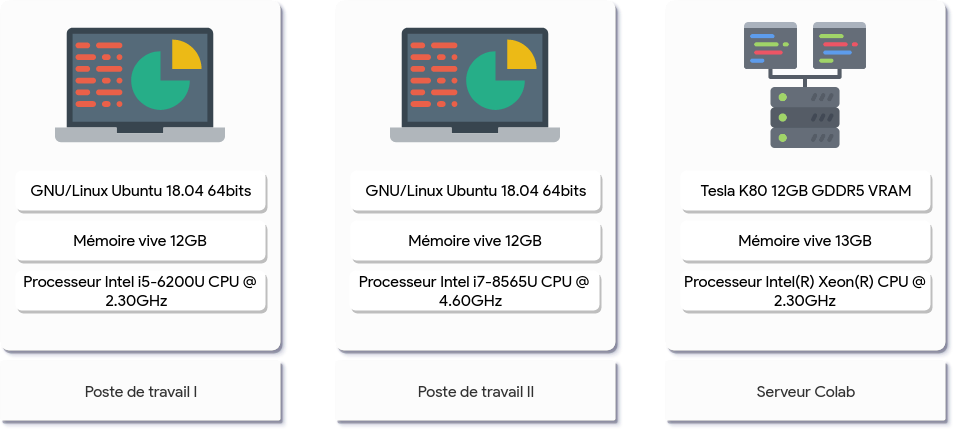
\includegraphics[width=0.88\linewidth]{images/implementation/machines.png}
		\caption{Caractéristiques des machines}
		\label{fig:machines}
		
	\end{figure}
	\par
	En ce qui concerne la partie logicielle, une liste non exhaustive est présentée ci dessous qui ne mentionne que les outils les plus utilisés et les plus exploités :
	\subsection{Langages de programmation}
%		\begin{figure}[H] 
%		\centering
%		
\includegraphics[width=0.3\linewidth]{images/implementation/langs.png}
%		\caption{Langages de programmation utilisés}
%		\label{fig:langs}
%	\end{figure}
		\subsubsection*{Python}
		\label{python}
		\paragraph{}
		 Python\footnote{\url{https://fr.wikibooks.org/wiki/Programmation_Python/Introduction}} est un langage de programmation interprété de haut niveau, structuré et open source. Il est multi-paradigme (orienté objet, programmation fonctionnelle et impérative) et multi-usage. Il est, comme la plupart des applications et outils open source, maintenu par une équipe de développeurs un peu partout dans le monde. Il offre une grande panoplie d'extensions (packages) pour résoudre une variété de problèmes, qu'ils soient liés au développement d'applications de bureau, web ou mobiles.
		
		\subsubsection*{Javascript} 
		\paragraph{}
		JavaScript\footnote{\url{https://fr.wikibooks.org/wiki/Programmation_JavaScript/Introduction}} est un langage de programmation utilisé principalement par les navigateurs web pour exécuter un bout de code incorporé dans une page web, plus communément appelé script. Il permet la manipulation de tous les éléments inclus dans une page, et par conséquent permet une gestion dynamique de ces derniers. Il est beaucoup utilisé du côté client mais peut aussi être exécuté du côté serveur. Tout comme Python, il offre une grande variété dans le choix des modules qui peuvent ajouter de nouvelles fonctionnalités, le tout géré par un gestionnaire de module \textit{npm} \footnote{Node Package Manager ou Gestionnaire de packages Node} devenu un standard.
	
	\subsection{Librairies et bibliothèques}
	\begin{figure}[H] 
		\centering
		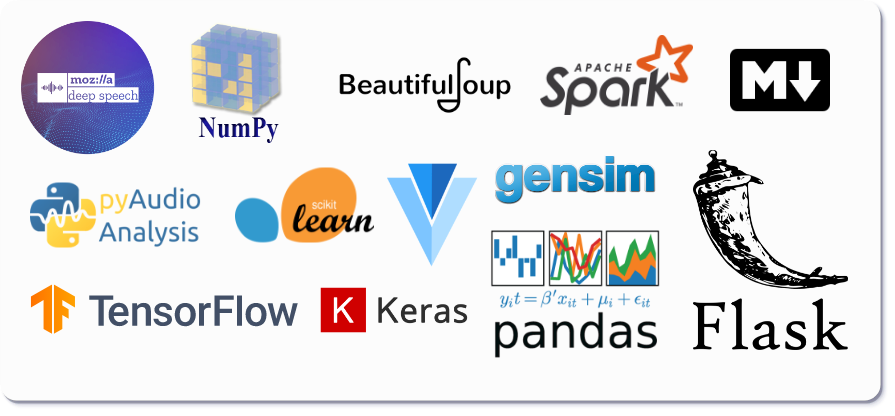
\includegraphics[width=0.9\linewidth]{images/implementation/libs_frams.png}
		\caption{Bibliothèques et librairies les plus utilisées dans ce projet.}
		\label{fig:libs_frams}
	\end{figure}
		\subsubsection*{DeepSpeech API}
		\paragraph{}
		C'est un module de python qui fait office d'interface entre un script Python et la librairie de reconnaissance automatique de la parole DeepSpeech \citep{deepspeech_paper}. Il permet entre autres de charger différents modèles acoustiques ou modèles de langues. Il offre aussi la possibilité d'utiliser des scripts d'apprentissage prédéfinis pour peu que les données soient organisées suivant une certaine norme; ces scripts sont notamment hautement paramétrables.
		\subsubsection*{PyAudio}
		\paragraph{}
		PyAudio\footnote{\url{https://pypi.org/project/PyAudio/}} est un librairie python destinée à la manipulation des fichiers ou flux audios. Elle offre entre autres la possibilité d'extraire des méta-données sur un flux audio (fréquence d'échantillonnage, débit, etc.). La possibilité d'extraire le vecteur de caractéristiques d'un extrait audio est aussi présente comme fonctionnalité.
		
		\subsubsection*{Beautiful Soup}
		\paragraph{}
		Beautiful Soup\footnote{\url{https://pypi.org/project/beautifulsoup4/}} est une bibliothèque Open source permettant l'analyse de fichiers html pour en extraire ou y injecter des données. Elle est principalement utilisée pour filtrer les balises html depuis une page web.
		
		\subsubsection*{PySpark}
		\paragraph{}
		PySpark\footnote{\url{https://spark.apache.org/}} est un package Python utilisé comme interface pour intéragir avec un serveur Spark. Il permet entre autres de lire et écrire des données dans le nouveau format Hadoop.
		
		\subsubsection*{Scikit-Learn}
		\paragraph{}
		Scikit-Learn\footnote{\url{https://scikit-learn.org/stable/}} est une bibliothèque Open source conçue pour rapidement développer des modèles pour l'apprentissage automatique, principalement utilisée pour ses nombreux outils de pré-traitement des données (codification, normalisation, filtrage ...).
		
		\subsubsection*{Numpy}
		\paragraph{}
		Numpy\footnote{\url{https://www.numpy.org/}} est une bibliothèque spécialisée dans la manipulation de grands volumes de données numériques, notamment les vecteurs (tableaux) multi-dimensionnels. Les opérations sur ces derniers sont implémentées en C pour optimiser au maximum leur coût en temps de calcul ou ressources mémoires utilisées. Elle offre des structures de données compatibles avec beaucoup d'autre librairies comme Tensorflow ou Keras.
		
		\subsubsection*{Tensorflow \& Keras}\label{tf&keras}
		\paragraph{}
		Tensorflow\footnote{\url{https://www.tensorflow.org/}} est une bibliothèque dédiée à l'apprentissage automatique, et plus particulièrement aux réseaux de neurones et l'apprentissage profond. Optimisée pour exécuter des opérations à grande échelle et massivement distribuées sur un réseau, Tensorflow offre la possibilité d'implémenter une grande variété d'architectures de modèles avec un maximum d'efficacité. Elle dispose d'un package Python permettant d'interagir avec le c\oe{}ur de la bibliothèque mais reste néanmoins assez bas-niveau. Keras\footnote{\url{https://keras.io/}} quant-à elle propose de rajouter une couche d'abstraction à Tensorflow. C'est un package python destiné à faciliter le développement de modèles pour l'apprentissage profond tout en offrant la possibilité de rajouter et modifier un grand nombre de fonctionnalités par défaut. Sa force réside dans le fait qu'il peut utiliser au plus bas niveau plusieurs librairies autres que Tensorflow comme Theano\footnote{\url{http://deeplearning.net/software/theano/}} et CNTK\footnote{\url{https://github.com/microsoft/CNTK}}.
		
		\subsubsection*{Flask}
		\paragraph{}
		Falsk\footnote{\url{http://flask.pocoo.org/}} est une micro-librairie Open source dédiée au développement d'applications basées web. De base, cette librairie est très légère, mais elle offre la possibilité d'ajouter des extensions qui s'intègrent très facilement au système de base.
		
		\subsubsection*{Vuetify}
		\paragraph{}
		Vuetify est une librairie Open source basée sur VueJs dédié au développement d'interfaces web ou mobiles. Elle implémente le paradigme Material Design de Google et offre la possibilité d'étendre les composants de base et de créer des interfaces belles et adaptatives.
	\subsection{Outils et logiciels de développement}
		\subsubsection*{PyCharm}
		\paragraph{}
		PyCharm est un environnement de développement intégré spécialisé et optimisé pour programmer dans le langage Python. Il permet l'analyse de code en continu et offre un débogueur intégré pour exécuter un code instruction par instruction. Il offre également l'intégration de logiciel de gestion de versions comme Git, et supporte le développement web avec Flask.
		
		\subsubsection*{Git}
		\paragraph{}
		Système décentralisé de gestion de versions. Il permet entre autres de gérer les différentes versions d'un projet durant son développement, mais aussi de garder l'historique des modifications effectuées ainsi que la possibilité de régler des conflits lors de l'intégration finale des contributions des développeurs.
		
		\subsubsection*{Google Colaboratory}
		\paragraph{}
		Colaboratory\footnote{\url{https://colab.research.google.com/}} est un outil de recherche et développement pour la formation et la recherche associées à l'apprentissage profond. C'est un environnement Python qui ne nécessite aucune configuration et offre la possibilité d'utiliser de puissantes machines rendues accessibles par Google pour accélérer la phase d'apprentissage.
		
		\subsubsection*{Protégé}
		\paragraph{}
		Protégé est un système dédié à la création et la modification d'ontologies. Il est développé en Java et est Open source distribué sous une licence libre (la Mozilla Public License). Il se démarque par le fait qu'il permet de travailler sur des ontologies de très grandes dimensions.
		
		
\section{Reconnaissance automatique de la parole}
\paragraph{}
Pour ce premier module, il a été très difficile d'effectuer les tests idéaux. En effet, nous n'avons pas pu trouver un ensemble de données qui proposait du contenu en rapport avec Speech2Act. Cependant, puisque nous avons pu construire un mini-ensemble pour tester l'apport de notre modèle de langue. Les résultats ne doivent pas être pris comme une référence absolue, mais plutôt comme une indication pour de possibles futurs tests.
	\subsection{Ensemble de test}
	\paragraph{}
	Pour tester le modèle acoustique, les données récoltées à travers le projet CommonVoice (voir la section \ref{common_voice}) constituent un assez bon échantillon, de par la nature des enregistrements (sur téléphone portable, par plusieurs genres et accents de locuteurs ...), mais aussi de par le volume (environs 500 heures d'enregistrements audios). Nous avons toutefois décidé de construire un mini-ensemble de test d'environ 204 enregistrements audios d'une longueur moyenne de 5 secondes chacun. Ces échantillons ont été prélevés sur trois locuteurs masculins. $20\%$ de ces échantillons ont été prélevés dans un environnement fermé mais bruité (il s'agit d'un espace de travail pour étudiants) et sur téléphone. Le reste a été prélevé dans un environnement fermé avec peu de bruit à partir du micro d'un ordinateur portable. Chaque enregistrement est soit : 
	\begin{itemize}
		\item une requête prélevée de l'ensemble de test du module de compréhension du langage naturel (voir les sections \ref{nlu_steps} et ~\ref{nlu_dataset}), ou
		
		\item une question prélevée de l'ensemble de données AskUbuntu\footnote{\url{https://github.com/taolei87/askubuntu}} qui regroupe des questions relatives à la manipulation d'un ordinateur sous le système d'exploitation GNU/Linux.
	\end{itemize}
	\par
	Pour le modèle de langue, il s'agit de celui mentionné dans la section 
	\ref{n-grams}. Quelques modifications ont été rajoutées comme le filtrage des mots qui n'appartiennent pas à la langue anglaise, mais au prix du sacrifice de quelques noms propres non reconnus ou bien de séquences de mots/lettres sans réel sens.
	\subsection{Méthodologie d'évaluation}
	\paragraph{}
	Les tests ont été effectués dans un serveur Colab pour libérer les machines locales. Les principales étapes sont les suivantes :  
	\begin{enumerate}
		\item \textbf{Préparation des données} : Les données sont prélevées d'une base de données sqlite qui comprend une seule table Transcriptions. Les colonnes de la table sont : 
		\begin{itemize}
			\item \textbf{id} : identifiant de l'enregistrement
			\item \textbf{path} : chemin vers le fichier audio de la requête.
			\item \textbf{text} : transcription textuelle de la requête.
		\end{itemize}
		\par
		Un script de conversion est ensuite lancé pour s'assurer que chaque enregistrement est au format .wav avec une fréquence de rafraîchissement égale à 16KHz, le modèle acoustique de DeepSpeech attend cette valeur exacte pour lancer l'inférence, sinon une erreur se produira.
		
		\item \textbf{Métriques retenues} : À chaque instance testée, le \textbf{WER} (Word Error Rate) est calculé. Pour rappel la formule du WER est la suivante :
		\begin{equation*}
			WER(y,\hat{y}) = \frac{S+D+I}{S+D+C} = \frac{S+D+I}{N}
		\end{equation*}
		où : 
		\begin{itemize}
			\item $\hat{y}$ est la séquence de mots prédite appelée Hypothèse.
			\item $y$ est la séquence de mots réelle appelée Référence.
			\item $S$ est le nombre de substitutions (compté en mots) réalisées entre l'hypothèse et la référence.
			\item $D$ est le nombre de suppressions qu'a effectué le système, donc le nombre de mots supprimés dans l'hypothèse par rapport à la référence.
			\item $I$ est le nombre d'insertions effectuées par le système (c.à.d. le nombre de mots rajoutés à l'hypothèse par rapport à la référence).
			\item $C$ est le nombre de mots bien placés.
			\item $N$ est la longueur totale de la séquence en nombre de mots
		\end{itemize}
		\item \textbf{Boucle d'évaluation} : L'opération précédente est réitérée en incrémentant à chaque fois le taux d'utilisation de notre modèle de langue (de 20\% à 100\% avec un pas de 10\%). Le WER associé est ensuite comparé à celui obtenu en utilisant le modèle de langue par défaut que propose DeepSpeech, le modèle acoustique sans modèle de langue, le résultat de l'API de Google \footnote{\url{https://cloud.google.com/speech-to-text/}} et enfin le modèle par défaut de CMU Sphinx \footnote{\url{https://cmusphinx.github.io/}}
		
	\end{enumerate}
	\subsection{Résultats}
	\paragraph{}
	Les résultats sont décrits dans le tableau \ref{tab:asr_results} et la figure \ref{fig:asr_results}. Nous remarquons que sur notre mini-ensemble de test, les modèles par défaut obtiennent un score très proche de 1, ce qui démontre qu'ils ont été entraînés sur des cas assez généraux, ce qui n'est pas très bon. Cependant, en changeant juste le modèle de langue par défaut en injectant des échantillons que nous avons récolté, une nette amélioration est visible (environ $-20\%$). Ce taux d'erreur diminue en augmentant la taille du corpus utilisé pour le modèle de langue. Toutefois, après avoir pris plus de $75\%$ du corpus, l'erreur a légèrement augmenté. Cela peut s'expliquer par la nature assez bruitée du corpus, les fichiers README.MD qui sont rédigés par des personnes, l'erreur humaine, et l'absence de processus de vérification de l'orthographe, de la grammaire ou de la syntaxe du contenu. Nous avions envisagé de choisir comme corpus des extraits de livres dédiés à la manipulation des ordinateurs sous Linux, mais nous n'avons pas trouvé de ressources gratuites ou Open source exploitables.
	\par
	Il est à noter que le meilleur résultat obtenu, c.à.d un taux d'erreur de $72.6\%$ est très loin d'être satisfaisant comparé au taux d'erreur de l'API de Google par exemple qui est d'approximativement $0.3496\%$. Néanmoins, l'ajout d'un modèle de langue personnalisé a pu améliorer nettement les résultats observés durant l'utilisation du modèle de base. Comme mentionné dans la section \ref{asr_probs}, DeepSpeech reste la meilleure option en Open Source à notre portée.
	\begin{table}[H]
		\centering
		\resizebox{\textwidth}{!}{%
			\begin{tabular}{c|c|}
				\cline{2-2}
				& WER (Word Error Rate) \\ \hline
				\multicolumn{1}{|c|}{Goole API} & 0,34955014 \\ \hline
				\multicolumn{1}{|c|}{Modèle acoustique avec 50\% du corpus} & 0,72634931 \\ \hline
				\multicolumn{1}{|c|}{Modèle acoustique avec 75\% du corpus} & 0,72809889 \\ \hline
				\multicolumn{1}{|c|}{Modèle acoustique avec 100\% du corpus} & 0,72928369 \\ \hline
				\multicolumn{1}{|c|}{Modèle acoustique avec 25\% du corpus} & 0,73910913 \\ \hline
				\multicolumn{1}{|c|}{Modèle acoustique avec 10\% du corpus} & 0,74333040 \\ \hline
				\multicolumn{1}{|c|}{Modèle acoustique et modèle de langue de base} & 0,79569078 \\ \hline
				\multicolumn{1}{|c|}{Modèle acoustique seulement} & 0,91092787 \\ \hline
				\multicolumn{1}{|c|}{CMU Sphinx de base} & 0,94024028 \\ \hline
			\end{tabular}%
		}
		\caption{Tableau récapitulatif des résultats pour le module de reconnaissance automatique de la parole.}
		\label{tab:asr_results}
	\end{table}
	\begin{figure}[H]
		\centering
		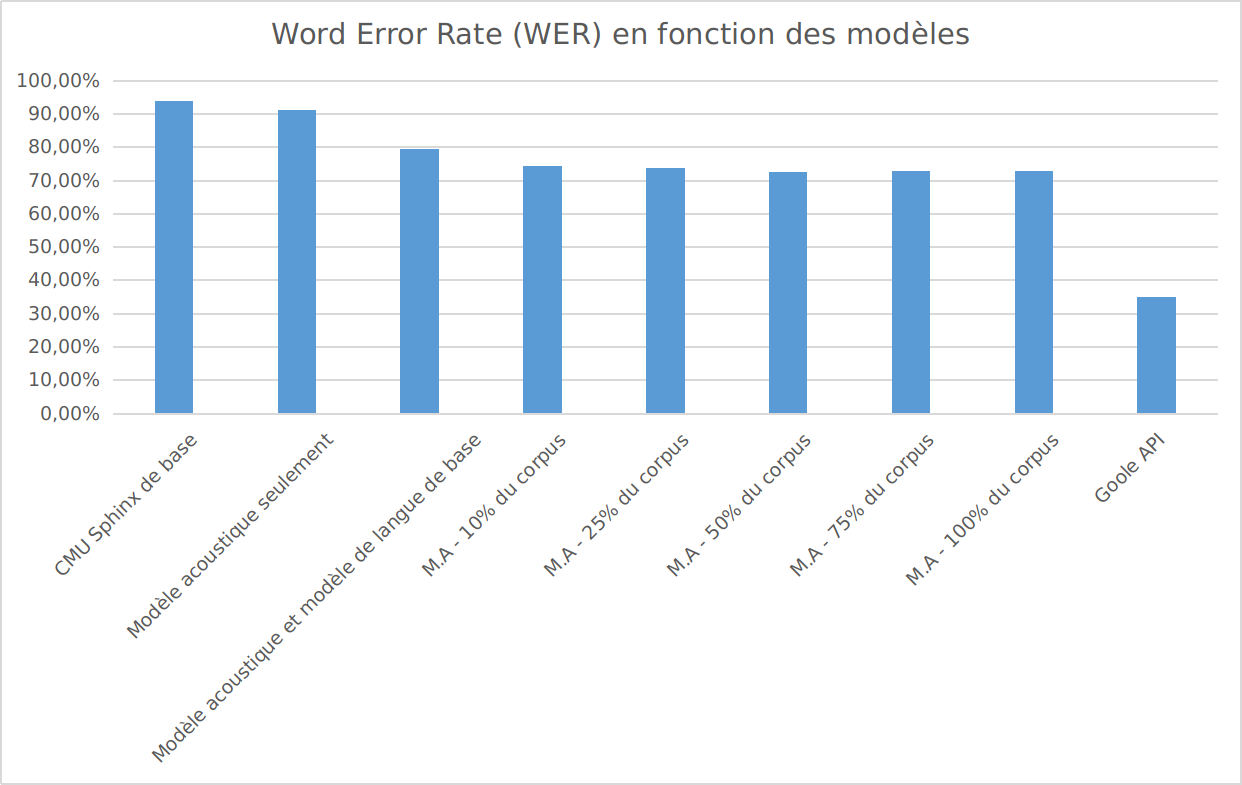
\includegraphics[width=.9\linewidth]{images/implementation/asr_graph.png} 
		\caption{Graphe récapitulatif des résultats pour le a reconnaissance automatique de la parole}
		\label{fig:asr_results}
	\end{figure}
\section{Classification d'intentions et extraction d'entités de domaine}
\paragraph{}
Pour ce module, une approche assez classique a été utilisée et l'ensemble de test est extrait de l'ensemble d'apprentissage (plus de détails dans la section suivante ). Les métriques d'évaluation utilisées sont mentionnées dans la sous section \ref{nlu_steps}. Nous commençons d'abord par détailler le contenu de l'ensemble de tests. Puis, nous présenterons la méthodologie suivie pour la réalisation de ces tests. Un tableau récapitulatif sera présenté avant la fin pour illustrer les différents résultats.
	\subsection{Ensemble de test}
	\paragraph{}
	Comme mentionné dans le chapitre précédent (voir la section \ref{nlu_dataset}), nous avons nous mêmes construit un ensemble d'apprentissage relativement varié. Il regroupe pour le moment essentiellement des commandes, ou requêtes liées à l'exploration de fichiers car c'est la tâche rudimentaire que Speech2Act peut accomplir.
	\par
	L'ensemble de test est dérivé de celui d'apprentissage selon une politique de découpage basée sur le taux de présence d'un intent (intention). Comme illustré dans la figure ~\ref{fig:split}, un pourcentage de chaque groupe d'instances affilié à la même classe est utilisé à la fois pour la validation et pour le test. Ce choix est motivé par le fait que les proportions des distributions des intentions dans l'ensemble original sont non-équilibrées.
	
	Une liste exhaustive des intentions et slots accompagnée d'une description est introduite dans le tableau \ref{tab:all_intents} ci dessous.
%	TODO insert table of intents and their tags
%	TODO figure here for ratio splitting  
	\begin{figure}[H]
		\centering
		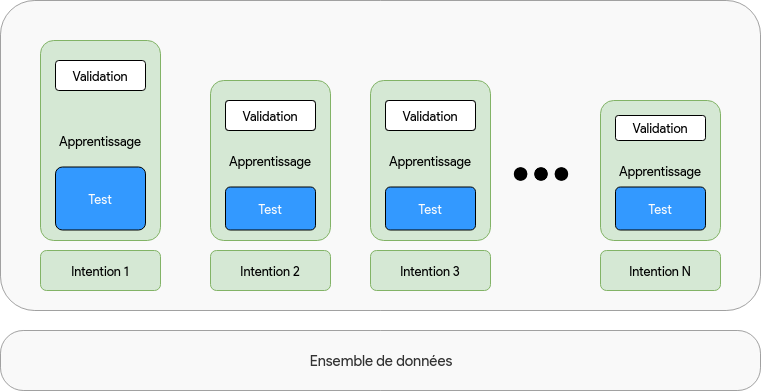
\includegraphics[width=.75\linewidth]{images/implementation/split.png} 
		\caption{Schéma de découpage des données pour l'apprentissage du modèle de compréhension du langage naturel} 
		\label{fig:split}
	\end{figure}

	\begin{table}[H]
		\centering
		\resizebox{\textwidth}{!}{%
			\begin{tabular}{|c|c|c|l|}
				\hline
				\textbf{Intention} & \textbf{\begin{tabular}[c]{@{}c@{}}Description \\ de l'intention\end{tabular}} & \textbf{Groupe} & \multicolumn{1}{c|}{\textbf{\begin{tabular}[c]{@{}c@{}}Argument(s)\\ ( Entité(s) )\end{tabular}}} \\ \hline
				create\_file\_desire & Création d'un fichier & ALTER & \begin{tabular}[c]{@{}l@{}}-file\_name\\ -parent\_directory\end{tabular} \\ \hline
				create\_directory\_desire & Création d'un répertoire & ALTER & \begin{tabular}[c]{@{}l@{}}-directory\_name\\ -parent\_directory\end{tabular} \\ \hline
				delete\_file\_desire & Suppression d'un fichier & ALTER & \begin{tabular}[c]{@{}l@{}}-file\_name\\ -parent\_directory\end{tabular} \\ \hline
				delete\_directory\_desire & Suppression d'un répertoire & ALTER & \begin{tabular}[c]{@{}l@{}}-directory\_name\\ -parent\_directory\end{tabular} \\ \hline
				open\_file\_desire & Ouverture d'un fichier & INFO & \begin{tabular}[c]{@{}l@{}}-file\_name\\ -parent\_directory\end{tabular} \\ \hline
				close\_file\_desire & Fermeture d'un fichier & INFO & \begin{tabular}[c]{@{}l@{}}-file\_name\\ -parent\_directory\end{tabular} \\ \hline
				copy\_file\_desire & Copie d'un fichier & ALTER & \begin{tabular}[c]{@{}l@{}}-file\_name\\ -origin\\ -destination\end{tabular} \\ \hline
				move\_file\_desire & Déplacement d'un fichier & ALTER & \begin{tabular}[c]{@{}l@{}}-file\_name\\ -origin\\ -destination\end{tabular} \\ \hline
				rename\_file\_desire & Renommage d'un fichier & - & \begin{tabular}[c]{@{}l@{}}-old\_name\\ -new\_name\end{tabular} \\ \hline
				change\_directory\_desire & \begin{tabular}[c]{@{}c@{}}Changement du répertoire \\ de travail courant\end{tabular} & - & -new\_directory \\ \hline
				inform & Informer d'une intention & EXCH & \begin{tabular}[c]{@{}l@{}}-file\_name\\ -parent\_directory\end{tabular} \\ \hline
				request & Demander une information & EXCH & \begin{tabular}[c]{@{}l@{}}-file\_name\\ -directory\end{tabular} \\ \hline
				deny & Réponse négative & - & \multicolumn{1}{c|}{-} \\ \hline
				confirm & Réponse positive & - & \multicolumn{1}{c|}{-} \\ \hline
				unknown & Intention inconnue & - & \multicolumn{1}{c|}{-} \\ \hline
			\end{tabular}%
		}
		\caption{Tableau récapitulatif de toutes les intentions avec leurs descriptions et leurs arguments.}
		\label{tab:all_intents}
	\end{table}
	\paragraph{}
	Les intentions sont regroupées en groupes; chaque groupe comporte des intentions qui influent sur les documents de la même manière. Il existe bien évidemment des intentions sans groupe, on peut considérer qu'ils forment un seul groupe, ou bien que chacun constitue son propre groupe : 
	\begin{itemize}
		\item \textbf{ALTER} : Groupe d'intentions qui altère l'état d'un document.
		\item \textbf{INFO} : Groupe d'intentions pour effectuer une opération puis informer l'utilisateur.
		\item \textbf{EXCH} : Groupe d'intentions dont le but est d'échanger des informations avec l'utilisateur.
	\end{itemize}
	\subsection{Méthodologie d'évaluation}
	\label{nlu_steps}
	\paragraph{}
	Après avoir construit l'ensemble de test, un parcours exhaustif des différentes combinaisons des paramètres suivants est effectué : 
	\begin{itemize}
		\item \textbf{Architecture d'encodage} :
		C'est à dire l'utilisation ou pas d'un réseau récurrent LSTM de base ou bien BiLSTM. Le but étant de montrer que le modèle pourra mieux interpréter les données en entrée s'il capture le contexte de chaque mot.
		
		\item \textbf{Nombre de neurones pour la couche de classification d'intention } : Lorsque l'encodeur retourne le dernier vecteur d'état caché, ce dernier passera par un réseau de neurones complètement connecté et multi-couches dont nombre de couches est fixé à 3 par souci de performance, une couche d'entrée, une couche intermédiaire et une couche de sortie. Le nombre de neurones sur la couche cachée dépend grandement de la complexité de la tâche à effectuer. La classification d'intentions pour l'exploration de fichier était relativement simple; nous avons commencé avec 32 neurones puis nous avons doublé ce nombre jusqu'à 512 pour, en théorie, donner plus de puissance au classificateur tout en évitant un sur-apprentissage par surplus de neurones.
		
		\item \textbf{Nombre d'unités d'une cellule LSTM (respectivement BiLSTM)}:
		Les portes d'une cellule LSTM (resp. BiLSTM) sont en vérité des réseaux de neurones denses (complètement connectés) et donc un ensemble de matrices de poids à optimiser. La capacité à "apprendre" la représentation des séquences dépend aussi du nombre de neurones dans ces mini-réseaux. Par le même raisonnement employé pour le classificateur d'intentions, nous avons commencé avec un petit nombre de neurones pour examiner d'une part où se trouverait le seuil minimal qui permettra au modèle de généraliser, et d'autre part où le seuil critique se situerait pour permettre au modèle de ne pas tomber dans un cas de sur-apprentissage. Nous partons de 128 jusqu'à 512 unités avec pas de 32 unités.
		
		\item \textbf{Fonctions d'activation} : 
		C'est un élément essentiel qui permet d'introduire la non-linéarité dans les relations entre chaque neurones de couches voisines. Ces fonctions permettent de mieux représenter les seuils d'activation des neurones. La fonction la plus utilisée dans la littérature est actuellement ReLu (Rectified Linear Unit) car elle a expérimentalement donné de meilleurs résultats dans une grande variété de tâches et problèmes liés à l'apprentissage automatique et à la classification et étiquetage de textes. Par souci d'exhaustivité, nous avons quand même décidé de tester deux autres fonctions $tanh$ (Tangente Hyperbolique) et $sigmoid$ (Sigmoïde). Pour chaque couche de sortie, la fonction $Softmax$ a été appliquée car chaque couche traite d'un problème de classification multi-classes. Voici les équations pour chacune de ces fonctions :
%		TODO equations for fucntions
		\begin{equation*}
			\tanh{x} = \frac{e^{x}-e^{-x}}{e^x+e^{-x}}
		\end{equation*}
		
		\begin{equation*}
			sigmoid(x) = \frac{1}{1+e^{-x}}
		\end{equation*}
		
		\begin{equation*}
			softmax_i(x) = \frac{e^{x_i}}{\sum_{j=1}^{K}e{^x_j}} \text{ pour } i=1,...,K \text{ et } x=(x_1,...,x_K) \in \mathbb{R}^K
		\end{equation*}
		\item \textbf{Fonction erreur}:
		C'est l'élément clé pour la phase d'apprentissage, cette fonction détermine le degré d'exactitude du modèle, c'est à dire à quel point il est proche de la bonne réponse. Nous avons décidé d'utiliser comme fonction erreur la fonction $Categorical\_Crossentropy$ ou Erreur Logistique; de par la nature de l'ensemble d'apprentissage et de test. Une version pondérée de cette fonction a été préférée, pour palier au problème du non équilibrage des classes, que ce soit pour la classification d'intentions, ou pour la reconnaissance d'entités du domaine.\\
		\par
		Les poids des classes sont calculés selon la formule suivante : 
		
		\begin{equation*}
			Poids_i = \max(1,\log{\frac{T}{T_i}})
		\end{equation*}
		où :
		\begin{itemize}
			\item  $T$ est le nombre total d'instances
			\item  $T_i$ est le nombre d'instances dont la classe est $C_i$
		\end{itemize}
		
		La formule de la fonction erreur devient donc : 
		\begin{equation*}
			Erreur(y,\hat{y}) = - \sum_{i}^{C} y_i * \log(\hat{y}_i) * Poids_i 
		\end{equation*}
		où : 
		\begin{itemize}
			\item $\hat{y}$ est le vecteur en sortie produit par le modèle à la suite d'une fonction $Softmax$.
			\item $y$ est le vecteur de classe réelle présent dans l'ensemble d'apprentissage
			\item $C$ est le nombre de classes au total.
		\end{itemize}
	
		\item \textbf{Fonction d'apprentissage}:
		Le choix de la fonction d'apprentissage est généralement affecté par un désir de précision et de rapidité. Une fonction qui converge rapidement en un minimum local peut être parfois préférée à une autre qui prendrait un temps considérable pour soit se retrouver dans le même minimum ou un autre minimum local (donc sans garantie de minimum optimal de la fonction erreur). Les deux fonctions utilisées sont RmsProp et Adam qui sont connues pour leur rapidité de convergence.
		
		\item \textbf{Encodage des entrée-sorties} :
		Là encore le choix de l'encodage des données influe grandement sur la capacité du modèle à distinguer et à représenter les différentes informations qui lui sont présentées. Comme initiative de notre part, nous avons mentionné dans la section \ref{nlu_dataset} l'ajout de l'étiquette morphosyntaxique de chaque mot à l'encodage. Nous avons donc lancé les tests sur un encodage avec et sans l'ajout des étiquettes pour mieux constater son impact.
		
		\item \textbf{Découpage des données} :
		La stratégie adoptée était de prendre aléatoirement les même proportions pour chaque sous-ensemble de chaque classe (intentions ou entités de domaine). Nous avons aussi décidé de faire varier les proportions de test et d'apprentissage en fixant celui de validation car nous avons remarqué que notre modèle n'arrivait pas à bien généraliser la relation entre les entrées et les sorties. Notre intuition portait sur le fait que le manque de données pouvait en être la cause (voir la section \ref{nlu_dataset} pour plus de détails). Ainsi, nous avons varié le taux de découpage pour les données de tests entre $25\%$ et $75\%$ avec un pas de $25\%$. Le taux de découpage pour les données de validations est fixé à $10\%$.
		\par
		Pour éviter que le modèle ne sur-apprenne, nous avons volontairement interchangé quelques mots dans la séquence d'entrée et celle de sortie pour introduire un certain taux d'erreur et de variété. Cet échange se fait suivant une probabilité $q$ fixée à $20\%$. Bien entendu, les étiquettes morphosyntaxiques ne sont pas échangées, et ce pour garder la structure de la phrase correcte.
	\end{itemize}
	\par
	Pour le reste des hyper-paramètres, la plupart ont été fixés par manque de temps et de ressources. Ainsi, le nombre d'epochs (itérations) a été limité au maximum à 15 avec une politique d'arrêt anticipé si la fonction erreur d'évaluation ne diminue pas plus d'un taux $\Delta E = 2*10^{-3}$ pendant au moins 4 itérations successives. Les métriques employées pour évaluer les deux classificateurs sont les suivantes : 
	\begin{itemize}
		\item \textbf{Précision} : il s'agit d'une métrique classique qui évalue à quel point le modèle est bon pour prédire les classes.
		\begin{equation*}
			P = \frac{VP}{VP+FP}
		\end{equation*}
		où : 
		\begin{itemize}
			\item $VP$ (Vrais Positifs) : nombre de cas où le modèle prédit correctement la classe comme étant positive.
			\item $FP$ (Faux Positifs) : nombre de cas où le modèle ne prédit pas correctement la classe comme étant positive.
		\end{itemize}

		\item \textbf{Rappel} : Cette métrique évalue la capacité du modèle à effectuer des classifications correctes par rapport à tout l'ensemble de test. Plus formellement : 
		\begin{equation*}
		R = \frac{VP}{VP+FN}
		\end{equation*}
		où : 
		\begin{itemize}
			\item $FN$ (Faux Négatifs) : nombre de cas où le modèle ne prédit pas correctement la classe comme étant négative.
		\end{itemize}
	
		\item \textbf{F-Mesure} : Mesure qui combine (d'une point de vue ensembliste) la précision et le rappel. Elle ne privilégie aucune des deux et essaye de donner un aperçu plus global de l'efficacité de l'algorithme en prenant compte des résultats de ces deux mesures.
		\begin{equation*}
		F-Mesure = \frac{2*R*P}{R+P}
		\end{equation*}
	\end{itemize}
	\subsection{Résultats}
	\paragraph{}
	Pour les résultats qui vont suivre, chaque tableau sera accompagné d'un paragraphe qui servira de commentaire aux résultats obtenus. Des remarques peuvent y être insérées pour attirer l'attention sur des détails non évidents.
	
	% Please add the following required packages to your document preamble:
	% \usepackage{graphicx}
	\begin{table}[H]
		\centering
		\resizebox{\textwidth}{!}{%
			\begin{tabular}{|c|c|c|c|c|c|c|c|c|}
				\hline
				\textbf{\begin{tabular}[c]{@{}c@{}}Nombre de\\ neurones\end{tabular}} & \textbf{\begin{tabular}[c]{@{}c@{}}Unités\\ LSTM\end{tabular}} & \textbf{Activation} & \textbf{Apprentissage} & \textbf{\begin{tabular}[c]{@{}c@{}}Précision\\ Intention\end{tabular}} & \textbf{\begin{tabular}[c]{@{}c@{}}Rappel\\ Intention\end{tabular}} & \textbf{\begin{tabular}[c]{@{}c@{}}Précision\\ Entités de\\ domaine\end{tabular}} & \textbf{\begin{tabular}[c]{@{}c@{}}Rappel\\ Entités de\\ domaine\end{tabular}} & \textbf{\begin{tabular}[c]{@{}c@{}}F-Mesure\\ moyenne\end{tabular}} \\ \hline
				32 & 128 & relu & rmsprop & 0,9743 & 0,9725 & 0,9214 & 0,9128 & 0,9452 \\ \hline
				32 & 256 & relu & rmsprop & 0,9755 & 0,9741 & 0,9066 & 0,8985 & 0,9387 \\ \hline
				32 & 512 & relu & rmsprop & 0,9750 & 0,9735 & 0,9082 & 0,9019 & 0,9396 \\ \hline
				64 & 128 & relu & rmsprop & 0,9700 & 0,9689 & 0,8744 & 0,8636 & 0,9192 \\ \hline
				64 & 256 & relu & rmsprop & 0,9753 & \textbf{0,9743} & 0,9141 & 0,9061 & 0,9424 \\ \hline
				\rowcolor[HTML]{96FFFB} 
				64 & 512 & relu & rmsprop & 0,9687 & 0,9669 & \textbf{0,9293} & 0,9230 & \textbf{0,9470} \\ \hline
				128 & 128 & relu & rmsprop & 0,9638 & 0,9626 & 0,8425 & 0,8283 & 0,8993 \\ \hline
				128 & 256 & relu & rmsprop & 0,9714 & 0,9707 & 0,8431 & 0,8345 & 0,9049 \\ \hline
				128 & 512 & relu & rmsprop & 0,9647 & 0,9635 & 0,8690 & 0,8584 & 0,9139 \\ \hline
				256 & 128 & relu & rmsprop & 0,9704 & 0,9692 & 0,8473 & 0,8342 & 0,9052 \\ \hline
				256 & 256 & relu & rmsprop & 0,7215 & 0,7141 & 0,7573 & 0,7275 & 0,7299 \\ \hline
				256 & 512 & relu & rmsprop & 0,9716 & 0,9711 & 0,8842 & 0,8761 & 0,9257 \\ \hline
			\end{tabular}%
		}
		\caption{Résultats des tests pour un encodage sans étiquetage morphosyntaxique avec des cellules LSTM avec découpage Apprentissage : 25\%, Validation : 10\%, Test : 75\%.}
		\label{tab:lstm_1}
	\end{table}
	
	\paragraph{}
	Nous pouvons remarquer depuis le tableau \ref{tab:lstm_1} que pour un ensemble d'apprentissage assez réduit, le modèle arrive tout de même à bien classifier la majorité des intentions avec un rappel maximum de $97,43\%$. Cependant, le slot-filling se révèle être une tâche plus ardue avec un rappel ne dépassant pas $92,30\%$. La meilleure combinaison qui équilibre les deux tâches utilise un petit nombre de neurones pour la classification d'intentions, mais en revanche demande une grande capacité de calcul pour la mémorisation des séquences en utilisant 512 unités dans les cellules LSTM.
	
	% Please add the following required packages to your document preamble:
	% \usepackage{graphicx}
	\begin{table}[H]
		\centering
		\resizebox{\textwidth}{!}{%
			\begin{tabular}{|c|c|c|c|c|c|c|c|c|}
				\hline
				\textbf{\begin{tabular}[c]{@{}c@{}}Nombre de\\ neurones\end{tabular}} & \textbf{\begin{tabular}[c]{@{}c@{}}Unités\\ LSTM\end{tabular}} & \textbf{Activation} & \textbf{Apprentissage} & \textbf{\begin{tabular}[c]{@{}c@{}}Précision\\ Intention\end{tabular}} & \textbf{\begin{tabular}[c]{@{}c@{}}Rappel\\ Intention\end{tabular}} & \textbf{\begin{tabular}[c]{@{}c@{}}Précision\\ Entités de\\ domaine\end{tabular}} & \textbf{\begin{tabular}[c]{@{}c@{}}Rappel\\ Entités de\\ domaine\end{tabular}} & \textbf{\begin{tabular}[c]{@{}c@{}}F-Mesure\\ moyenne\end{tabular}} \\ \hline
				32 & 128 & relu & rmsprop & 0,9736 & 0,9721 & 0,8894 & 0,8817 & 0,9292 \\ \hline
				32 & 256 & relu & rmsprop & 0,9746 & 0,9735 & 0,9344 & 0,9298 & 0,9531 \\ \hline
				32 & 512 & relu & rmsprop & 0,9721 & 0,9714 & 0,9149 & 0,9089 & 0,9418 \\ \hline
				64 & 128 & relu & rmsprop & 0,9687 & 0,9684 & 0,9344 & 0,9286 & 0,9500 \\ \hline
				64 & 256 & relu & rmsprop & 0,9737 & 0,9729 & 0,9389 & 0,9325 & 0,9545 \\ \hline
				64 & 512 & relu & rmsprop & 0,9741 & 0,9732 & 0,9257 & 0,9188 & 0,9479 \\ \hline
				\rowcolor[HTML]{96FFFB} 
				128 & 128 & relu & rmsprop & 0,9684 & 0,9674 & 0,9354 & 0,9299 & \textbf{0,9503} \\ \hline
				128 & 256 & relu & rmsprop & 0,9709 & 0,9703 & 0,9360 & 0,9304 & 0,9519 \\ \hline
				128 & 512 & relu & rmsprop & 0,9749 & 0,9736 & 0,9426 & \textbf{0,9380} & 0,9573 \\ \hline
				256 & 128 & relu & rmsprop & 0,9681 & 0,9673 & 0,9349 & 0,9286 & 0,9497 \\ \hline
				256 & 256 & relu & rmsprop & 0,9686 & 0,9679 & 0,9048 & 0,8995 & 0,9352 \\ \hline
				256 & 512 & relu & rmsprop & 0,9768 & \textbf{0,9762} & 0,9272 & 0,9221 & 0,9505 \\ \hline
			\end{tabular}%
		}
		\caption{Résultats des tests pour un encodage sans étiquetage morphosyntaxique avec des cellules BiLSTM avec découpage Apprentissage : 25\%, Validation : 10\%, Test : 75\%.}
		\label{tab:bilstm_1}
	\end{table}
	
	\paragraph{}
	Dans le tableau \ref{tab:bilstm_1}, l'ajout de l'information du contexte pour un mot à une position donnée à travers l'utilisation d'une architecture BiLSTM affecte systématiquement les scores (Précision, Rappel et F-Mesure). Ceux-ci augmentent d'un certain taux ($\approx 10\%$) dans la majorité des cas. Il est a noter que pour le même nombre d'unités BiLSTM, le nombre de neurones pour la classification d'intentions a doublé.
	
	
	
	\begin{table}[H]
		\centering
		\resizebox{\textwidth}{!}{%
			\begin{tabular}{|c|c|c|c|c|c|c|c|c|}
				\hline
				\textbf{\begin{tabular}[c]{@{}c@{}}Nombre de\\ neurones\end{tabular}} & \textbf{\begin{tabular}[c]{@{}c@{}}Unités\\ LSTM\end{tabular}} & \textbf{Activation} & \textbf{Apprentissage} & \textbf{\begin{tabular}[c]{@{}c@{}}Précision\\ Intention\end{tabular}} & \textbf{\begin{tabular}[c]{@{}c@{}}Rappel\\ Intention\end{tabular}} & \textbf{\begin{tabular}[c]{@{}c@{}}Précision\\ Entités de\\ domaine\end{tabular}} & \textbf{\begin{tabular}[c]{@{}c@{}}Rappel\\ Entités de\\ domaine\end{tabular}} & \textbf{\begin{tabular}[c]{@{}c@{}}F-Mesure\\ moyenne\end{tabular}} \\ \hline
				32 & 128 & relu & rmsprop & 0,9769 & 0,9738 & 0,9189 & 0,9115 & 0,9453 \\ \hline
				32 & 256 & relu & rmsprop & 0,9703 & 0,9693 & 0,8609 & 0,8513 & 0,9129 \\ \hline
				32 & 512 & relu & rmsprop & 0,9717 & 0,9706 & 0,9304 & 0,9238 & 0,9491 \\ \hline
				64 & 128 & relu & rmsprop & 0,9696 & 0,9672 & 0,8556 & 0,8465 & 0,9097 \\ \hline
				\rowcolor[HTML]{96FFFB} 
				64 & 256 & relu & rmsprop & 0,969 & 0,9686 & 0,9354 & \textbf{0,9287} & \textbf{0,9504} \\ \hline
				64 & 512 & relu & rmsprop & 0,9761 & \textbf{0,9750} & 0,8275 & 0,8201 & 0,8997 \\ \hline
				128 & 128 & relu & rmsprop & 0,9713 & 0,9695 & 0,8565 & 0,8455 & 0,9107 \\ \hline
				128 & 256 & relu & rmsprop & 0,9689 & 0,9681 & 0,9204 & 0,9131 & 0,9426 \\ \hline
				128 & 512 & relu & rmsprop & 0,9714 & 0,9708 & 0,8756 & 0,8693 & 0,9218 \\ \hline
				256 & 128 & relu & rmsprop & 0,9707 & 0,9699 & 0,8767 & 0,8674 & 0,9212 \\ \hline
				256 & 256 & relu & rmsprop & 0,965 & 0,9642 & 0,8767 & 0,8707 & 0,9191 \\ \hline
				256 & 512 & relu & rmsprop & 0,9751 & 0,9739 & 0,8418 & 0,8291 & 0,905 \\ \hline
			\end{tabular}%
		}
		\caption{Résultats des tests pour un encodage avec étiquetage morphosyntaxique avec des cellules LSTM avec découpage Apprentissage : 25\%, Validation : 10\%, Test : 75\%.}
		\label{tab:lstm_1_postag}
	\end{table}
	\begin{table}[H]
		\centering
		\resizebox{\textwidth}{!}{%
			\begin{tabular}{|c|c|c|c|c|c|c|c|c|}
				\hline
				\textbf{\begin{tabular}[c]{@{}c@{}}Nombre de\\ neurones\end{tabular}} & \textbf{\begin{tabular}[c]{@{}c@{}}Unités\\ LSTM\end{tabular}} & \textbf{Activation} & \textbf{Apprentissage} & \textbf{\begin{tabular}[c]{@{}c@{}}Précision\\ Intention\end{tabular}} & \textbf{\begin{tabular}[c]{@{}c@{}}Rappel\\ Intention\end{tabular}} & \textbf{\begin{tabular}[c]{@{}c@{}}Précision\\ Entités de\\ domaine\end{tabular}} & \textbf{\begin{tabular}[c]{@{}c@{}}Rappel\\ Entités de\\ domaine\end{tabular}} & \textbf{\begin{tabular}[c]{@{}c@{}}F-Mesure\\ moyenne\end{tabular}} \\ \hline
				32 & 128 & relu & rmsprop & 0,9726 & 0,9708 & 0,93 & 0,9232 & 0,9491 \\ \hline
				\rowcolor[HTML]{96FFFB} 
				32 & 256 & relu & rmsprop & 0,9726 & 0,9715 & 0,9481 & \textbf{0,9436} & \textbf{0,9589} \\ \hline
				32 & 512 & relu & rmsprop & 0,9683 & 0,9656 & 0,9392 & 0,933 & 0,9515 \\ \hline
				64 & 128 & relu & rmsprop & 0,9735 & 0,9719 & 0,8369 & 0,8278 & 0,9025 \\ \hline
				64 & 256 & relu & rmsprop & 0,9735 & 0,9731 & 0,937 & 0,9329 & 0,9541 \\ \hline
				64 & 512 & relu & rmsprop & 0,9651 & 0,9636 & 0,9324 & 0,9261 & 0,9468 \\ \hline
				128 & 128 & relu & rmsprop & 0,9702 & 0,9687 & 0,8721 & 0,867 & 0,9195 \\ \hline
				128 & 256 & relu & rmsprop & 0,9741 & 0,9732 & 0,8209 & 0,8114 & 0,8949 \\ \hline
				128 & 512 & relu & rmsprop & 0,9794 & \textbf{0,979} & 0,923 & 0,9163 & 0,9494 \\ \hline
				256 & 128 & relu & rmsprop & 0,9654 & 0,9645 & 0,9324 & 0,9266 & 0,9472 \\ \hline
				256 & 256 & relu & rmsprop & 0,9682 & 0,967 & 0,9394 & 0,9352 & 0,9525 \\ \hline
				256 & 512 & relu & rmsprop & 0,9733 & 0,9723 & 0,9357 & 0,9304 & 0,9529 \\ \hline
			\end{tabular}%
		}
		\caption{Résultats des tests pour un encodage avec étiquetage morphosyntaxique avec des cellules BiLSTM avec découpage Apprentissage : 25\%, Validation : 10\%, Test : 75\%.}
		\label{tab:bilstm_1_postag}
	\end{table}
	
	\paragraph{}
	Quant-aux deux tableaux \ref{tab:lstm_1_postag} et \ref{tab:bilstm_1_postag}, ils montrent que l'ajout de l'étiquette morphosyntaxique a amélioré les résultats pour cas de l'utilisation d'une cellule LSTM simple tout en réduisant le nombre d'unités requises, moins de calculs et plus d'efficacité. Cela se confirme encore plus pour le cas de l'utilisation de l'architecture BiLSTM, en réduisant de presque la moitié la puissance de calcul nécessaire et en augmentant un tout petit peu la qualité des prédictions.
	
	
	
	
%	----------------------------------------------------------------------- %
%POSTAGS
		% Please add the following required packages to your document preamble:
	% \usepackage{graphicx}
	\begin{table}[H]
		\centering
		\resizebox{\textwidth}{!}{%
			\begin{tabular}{|c|c|c|c|c|c|c|c|c|}
				\hline
				\textbf{\begin{tabular}[c]{@{}c@{}}Nombre de\\ neurones\end{tabular}} & \textbf{\begin{tabular}[c]{@{}c@{}}Unités\\ LSTM\end{tabular}} & \textbf{Activation} & \textbf{Apprentissage} & \textbf{\begin{tabular}[c]{@{}c@{}}Précision\\ Intention\end{tabular}} & \textbf{\begin{tabular}[c]{@{}c@{}}Rappel\\ Intention\end{tabular}} & \textbf{\begin{tabular}[c]{@{}c@{}}Précision\\ Entités de\\ domaine\end{tabular}} & \textbf{\begin{tabular}[c]{@{}c@{}}Rappel\\ Entités de\\ domaine\end{tabular}} & \textbf{\begin{tabular}[c]{@{}c@{}}F-Mesure\\ moyenne\end{tabular}} \\ \hline
				32 & 128 & relu & rmsprop & 0,9707 & 0,9691 & 0,8897 & 0,8776 & 0,9267 \\ \hline
				32 & 256 & relu & rmsprop & 0,974 & 0,9724 & 0,8921 & 0,8859 & 0,9311 \\ \hline
				32 & 512 & relu & rmsprop & 0,9708 & 0,9699 & 0,9293 & 0,9222 & 0,948 \\ \hline
				64 & 128 & relu & rmsprop & 0,9751 & 0,9729 & 0,8901 & 0,8796 & 0,9294 \\ \hline
				64 & 256 & relu & rmsprop & 0,9706 & 0,9698 & 0,9096 & 0,903 & 0,9383 \\ \hline
				\rowcolor[HTML]{96FFFB} 
				64 & 512 & relu & rmsprop & 0,9717 & 0,9708 & 0,934 & 0,9262 & \textbf{0,9506} \\ \hline
				128 & 128 & relu & rmsprop & 0,965 & 0,9633 & 0,8212 & 0,8081 & 0,8894 \\ \hline
				128 & 256 & relu & rmsprop & 0,9712 & 0,9706 & 0,893 & 0,8817 & 0,9291 \\ \hline
				128 & 512 & relu & rmsprop & 0,9711 & 0,9698 & 0,9316 & \textbf{0,9269} & 0,9498 \\ \hline
				256 & 128 & relu & rmsprop & 0,9749 & \textbf{0,9741} & 0,9079 & 0,8988 & 0,9389 \\ \hline
				256 & 256 & relu & rmsprop & 0,9718 & 0,9712 & 0,8629 & 0,8555 & 0,9153 \\ \hline
				256 & 512 & relu & rmsprop & 0,9728 & 0,9725 & 0,93 & 0,9239 & 0,9498 \\ \hline
			\end{tabular}%
		}
		\caption{Résultats des tests pour un encodage sans étiquetage morphosyntaxique avec des cellules LSTM avec découpage Apprentissage : 50\%, Validation : 10\%, Test : 50\%.}
		\label{tab:lstm_2}
	\end{table}
	
	\begin{table}[H]
		\centering
		\resizebox{\textwidth}{!}{%
			\begin{tabular}{|c|c|c|c|c|c|c|c|c|}
				\hline
				\textbf{\begin{tabular}[c]{@{}c@{}}Nombre de\\ neurones\end{tabular}} & \textbf{\begin{tabular}[c]{@{}c@{}}Unités\\ LSTM\end{tabular}} & \textbf{Activation} & \textbf{Apprentissage} & \textbf{\begin{tabular}[c]{@{}c@{}}Précision\\ Intention\end{tabular}} & \textbf{\begin{tabular}[c]{@{}c@{}}Rappel\\ Intention\end{tabular}} & \textbf{\begin{tabular}[c]{@{}c@{}}Précision\\ Entités de\\ domaine\end{tabular}} & \textbf{\begin{tabular}[c]{@{}c@{}}Rappel\\ Entités de\\ domaine\end{tabular}} & \textbf{\begin{tabular}[c]{@{}c@{}}F-Mesure\\ moyenne\end{tabular}} \\ \hline
				32 & 128 & relu & rmsprop & 0,9539 & 0,948 & 0,8215 & 0,8064 & 0,8824 \\ \hline
				32 & 256 & relu & rmsprop & 0,9649 & 0,9629 & 0,8947 & 0,8887 & 0,9278 \\ \hline
				32 & 512 & relu & rmsprop & 0,9689 & 0,9673 & 0,9456 & \textbf{0,9409} & 0,9557 \\ \hline
				64 & 128 & relu & rmsprop & 0,9679 & 0,9667 & 0,8941 & 0,8879 & 0,9291 \\ \hline
				\rowcolor[HTML]{96FFFB} 
				64 & 256 & relu & rmsprop & 0,974 & 0,9732 & 0,9425 & 0,9369 & \textbf{0,9567} \\ \hline
				64 & 512 & relu & rmsprop & 0,9771 & \textbf{0,9762} & 0,9339 & 0,9302 & 0,9543 \\ \hline
				128 & 128 & relu & rmsprop & 0,9699 & 0,9693 & 0,9326 & 0,9264 & 0,9496 \\ \hline
				128 & 256 & relu & rmsprop & 0,9654 & 0,9645 & 0,9384 & 0,9328 & 0,9503 \\ \hline
				128 & 512 & relu & rmsprop & 0,8747 & 0,8657 & 0,7848 & 0,7628 & 0,8219 \\ \hline
				256 & 128 & relu & rmsprop & 0,971 & 0,97 & 0,7782 & 0,7656 & 0,8712 \\ \hline
				256 & 256 & relu & rmsprop & 0,9716 & 0,9711 & 0,9327 & 0,9266 & 0,9505 \\ \hline
				256 & 512 & relu & rmsprop & 0,9752 & 0,9745 & 0,939 & 0,9326 & 0,9553 \\ \hline
			\end{tabular}%
		}
		\caption{Résultats des tests pour un encodage sans étiquetage morphosyntaxique avec des cellules BiLSTM avec découpage Apprentissage : 50\%, Validation : 10\%, Test : 50\%.}
		\label{tab:bilstm_2}
	\end{table}
	
	
	\paragraph{}
	D'après les résultats des tableaux \ref{tab:lstm_2} et \ref{tab:bilstm_2}, le choix de l'architecture BiLSTM à amélioré la qualité des classifications, même si ce n'est que d'un petit taux. Ces tableaux semblent aussi montrer que notre intuition sur la faible quantité de données que nous possédions soit fondée. Les scores de F-Mesure tendent en moyenne à augmenter avec l'injection de nouvelles données d'apprentissage.
	
	\begin{table}[H]
		\centering
		\resizebox{\textwidth}{!}{%
			\begin{tabular}{|c|c|c|c|c|c|c|c|c|}
				\hline
				\textbf{\begin{tabular}[c]{@{}c@{}}Nombre de\\ neurones\end{tabular}} & \textbf{\begin{tabular}[c]{@{}c@{}}Unités\\ LSTM\end{tabular}} & \textbf{Activation} & \textbf{Apprentissage} & \textbf{\begin{tabular}[c]{@{}c@{}}Précision\\ Intention\end{tabular}} & \textbf{\begin{tabular}[c]{@{}c@{}}Rappel\\ Intention\end{tabular}} & \textbf{\begin{tabular}[c]{@{}c@{}}Précision\\ Entités de\\ domaine\end{tabular}} & \textbf{\begin{tabular}[c]{@{}c@{}}Rappel\\ Entités de\\ domaine\end{tabular}} & \textbf{\begin{tabular}[c]{@{}c@{}}F-Mesure\\ moyenne\end{tabular}} \\ \hline
				32 & 128 & relu & rmsprop & 0,9729 & 0,9712 & 0,9256 & 0,9182 & 0,9469 \\ \hline
				32 & 256 & relu & rmsprop & 0,9734 & 0,9716 & 0,8769 & 0,8689 & 0,9227 \\ \hline
				32 & 512 & relu & rmsprop & 0,9692 & 0,9681 & 0,9278 & 0,9226 & 0,9469 \\ \hline
				64 & 128 & relu & rmsprop & 0,9712 & 0,9693 & 0,8732 & 0,8641 & 0,9195 \\ \hline
				64 & 256 & relu & rmsprop & 0,9720 & 0,9709 & 0,9278 & 0,9219 & 0,9482 \\ \hline
				64 & 512 & relu & rmsprop & 0,9689 & 0,9671 & 0,9187 & 0,9107 & 0,9414 \\ \hline
				128 & 128 & relu & rmsprop & 0,9631 & 0,9614 & 0,8223 & 0,8090 & 0,8889 \\ \hline
				128 & 256 & relu & rmsprop & 0,9694 & 0,9686 & 0,8020 & 0,7936 & 0,8834 \\ \hline
				\rowcolor[HTML]{96FFFB} 
				128 & 512 & relu & rmsprop & 0,9723 & 0,9716 & 0,9388 & \textbf{0,9330} & \textbf{0,9539} \\ \hline
				256 & 128 & relu & rmsprop & 0,9662 & 0,9655 & 0,8661 & 0,8563 & 0,9135 \\ \hline
				256 & 256 & relu & rmsprop & 0,9702 & 0,9699 & 0,9077 & 0,9016 & 0,9373 \\ \hline
				256 & 512 & relu & rmsprop & 0,9737 & \textbf{0,9731} & 0,9238 & 0,9193 & 0,9475 \\ \hline
			\end{tabular}%
		}
		\caption{Résultats des tests pour un encodage avec étiquetage morphosyntaxique avec des cellules LSTM avec découpage Apprentissage : 50\%, Validation : 10\%, Test : 50\%.}
		\label{tab:lstm_2_postag}
	\end{table}

	\begin{table}[H]
		\centering
		\resizebox{\textwidth}{!}{%
			\begin{tabular}{|c|c|c|c|c|c|c|c|c|}
				\hline
				\textbf{\begin{tabular}[c]{@{}c@{}}Nombre de\\ neurones\end{tabular}} & \textbf{\begin{tabular}[c]{@{}c@{}}Unités\\ LSTM\end{tabular}} & \textbf{Activation} & \textbf{Apprentissage} & \textbf{\begin{tabular}[c]{@{}c@{}}Précision\\ Intention\end{tabular}} & \textbf{\begin{tabular}[c]{@{}c@{}}Rappel\\ Intention\end{tabular}} & \textbf{\begin{tabular}[c]{@{}c@{}}Précision\\ Entités de\\ domaine\end{tabular}} & \textbf{\begin{tabular}[c]{@{}c@{}}Rappel\\ Entités de\\ domaine\end{tabular}} & \textbf{\begin{tabular}[c]{@{}c@{}}F-Mesure\\ moyenne\end{tabular}} \\ \hline
				32 & 128 & relu & rmsprop & 0,9906 & 0,9900 & 0,9559 & 0,9524 & 0,9722 \\ \hline
				\rowcolor[HTML]{96FFFB} 
				32 & 256 & relu & rmsprop & 0,9920 & 0,9914 & 0,9650 & 0,9623 & \textbf{0,9777} \\ \hline
				32 & 512 & relu & rmsprop & 0,9900 & 0,9894 & 0,9603 & 0,9577 & 0,9744 \\ \hline
				64 & 128 & relu & rmsprop & 0,9903 & 0,9903 & 0,9621 & 0,9594 & 0,9755 \\ \hline
				64 & 256 & relu & rmsprop & 0,9871 & 0,9870 & 0,9570 & 0,9539 & 0,9713 \\ \hline
				64 & 512 & relu & rmsprop & 0,9893 & 0,9886 & 0,9604 & 0,9579 & 0,9741 \\ \hline
				128 & 128 & relu & rmsprop & 0,9935 & \textbf{0,9931} & 0,9581 & 0,9550 & 0,9749 \\ \hline
				128 & 256 & relu & rmsprop & 0,9885 & 0,9883 & 0,8658 & 0,8610 & 0,9259 \\ \hline
				128 & 512 & relu & rmsprop & 0,9896 & 0,9889 & 0,9619 & 0,9591 & 0,9749 \\ \hline
				256 & 128 & relu & rmsprop & 0,9878 & 0,9877 & 0,9518 & 0,9481 & 0,9689 \\ \hline
				256 & 256 & relu & rmsprop & 0,9882 & 0,9875 & 0,9016 & 0,8959 & 0,9433 \\ \hline
				256 & 512 & relu & rmsprop & 0,9883 & 0,9879 & 0,9652 & \textbf{0,9625} & 0,9760 \\ \hline
			\end{tabular}%
		}
		\caption{Résultats des tests pour un encodage avec étiquetage morphosyntaxique avec des cellules BiLSTM avec découpage Apprentissage : 50\%, Validation : 10\%, Test : 50\%.}
		\label{tab:bilstm_2_postag}
	\end{table}
	\paragraph{}
	Pour les tableaux \ref{tab:lstm_2_postag} et \ref{tab:bilstm_2_postag}, nous pouvons observer que l'ajout de l'information morphosyntaxique a amélioré le taux de réussite de la prédiction d'un faible taux au profit d'une moindre puissance de calculs.
	
%75 10 25

	\begin{table}[H]
		\centering
		\resizebox{\textwidth}{!}{%
			\begin{tabular}{|c|c|c|c|c|c|c|c|c|}
				\hline
				\textbf{\begin{tabular}[c]{@{}c@{}}Nombre de\\ neurones\end{tabular}} & \textbf{\begin{tabular}[c]{@{}c@{}}Unités\\ LSTM\end{tabular}} & \textbf{Activation} & \textbf{Apprentissage} & \textbf{\begin{tabular}[c]{@{}c@{}}Précision\\ Intention\end{tabular}} & \textbf{\begin{tabular}[c]{@{}c@{}}Rappel\\ Intention\end{tabular}} & \textbf{\begin{tabular}[c]{@{}c@{}}Précision\\ Entités de\\ domaine\end{tabular}} & \textbf{\begin{tabular}[c]{@{}c@{}}Rappel\\ Entités de\\ domaine\end{tabular}} & \textbf{\begin{tabular}[c]{@{}c@{}}F-Mesure\\ moyenne\end{tabular}} \\ \hline
				32 & 128 & relu & rmsprop & 0,9873 & 0,9869 & 0,9556 & 0,9518 & 0,9704 \\ \hline
				32 & 256 & relu & rmsprop & 0,9871 & 0,9869 & 0,9616 & 0,9589 & 0,9736 \\ \hline
				32 & 512 & relu & rmsprop & 0,9914 & \textbf{0,9913} & 0,9618 & 0,9588 & 0,9758 \\ \hline
				64 & 128 & relu & rmsprop & 0,9896 & 0,9896 & 0,9520 & 0,9477 & 0,9697 \\ \hline
				64 & 256 & relu & rmsprop & 0,9904 & 0,9904 & 0,9629 & \textbf{0,9600} & 0,9760 \\ \hline
				64 & 512 & relu & rmsprop & 0,9894 & 0,9894 & 0,9519 & 0,9479 & 0,9696 \\ \hline
				128 & 128 & relu & rmsprop & 0,9874 & 0,9874 & 0,9263 & 0,9204 & 0,9554 \\ \hline
				\rowcolor[HTML]{96FFFB} 
				128 & 256 & relu & rmsprop & 0,9916 & 0,9897 & 0,9628 & 0,9600 & \textbf{0,9760} \\ \hline
				128 & 512 & relu & rmsprop & 0,9885 & 0,9883 & 0,9581 & 0,9548 & 0,9724 \\ \hline
				256 & 128 & relu & rmsprop & 0,9803 & 0,9792 & 0,9105 & 0,9014 & 0,9429 \\ \hline
				256 & 256 & relu & rmsprop & 0,9906 & 0,9906 & 0,9509 & 0,9470 & 0,9698 \\ \hline
				256 & 512 & relu & rmsprop & 0,9901 & 0,9892 & 0,9607 & 0,9576 & 0,9744 \\ \hline
			\end{tabular}%
		}
		\caption{Résultats des tests pour un encodage sans étiquetage morphosyntaxique avec des cellules LSTM avec découpage Apprentissage : 75\%, Validation : 10\%, Test : 25\%.}
		\label{tab:lstm_3}
	\end{table}
	
	\begin{table}[H]
		\centering
		\resizebox{\textwidth}{!}{%
			\begin{tabular}{|c|c|c|c|c|c|c|c|c|}
				\hline
				\textbf{\begin{tabular}[c]{@{}c@{}}Nombre de\\ neurones\end{tabular}} & \textbf{\begin{tabular}[c]{@{}c@{}}Unités\\ LSTM\end{tabular}} & \textbf{Activation} & \textbf{Apprentissage} & \textbf{\begin{tabular}[c]{@{}c@{}}Précision\\ Intention\end{tabular}} & \textbf{\begin{tabular}[c]{@{}c@{}}Rappel\\ Intention\end{tabular}} & \textbf{\begin{tabular}[c]{@{}c@{}}Précision\\ Entités de\\ domaine\end{tabular}} & \textbf{\begin{tabular}[c]{@{}c@{}}Rappel\\ Entités de\\ domaine\end{tabular}} & \textbf{\begin{tabular}[c]{@{}c@{}}F-Mesure\\ moyenne\end{tabular}} \\ \hline
				32 & 128 & relu & rmsprop & 0,9889 & 0,9887 & 0,9626 & 0,9601 & 0,9750 \\ \hline
				32 & 256 & relu & rmsprop & 0,9865 & 0,9865 & 0,9611 & 0,9571 & 0,9728 \\ \hline
				32 & 512 & relu & rmsprop & 0,9862 & 0,9846 & 0,9622 & 0,9597 & 0,9732 \\ \hline
				64 & 128 & relu & rmsprop & 0,9868 & 0,9866 & 0,9627 & 0,9598 & 0,9740 \\ \hline
				64 & 256 & relu & rmsprop & 0,9869 & 0,9856 & 0,8581 & 0,8504 & 0,9202 \\ \hline
				64 & 512 & relu & rmsprop & 0,9872 & 0,9871 & 0,9650 & 0,9626 & 0,9755 \\ \hline
				128 & 128 & relu & rmsprop & 0,9779 & 0,9779 & 0,9609 & 0,9580 & 0,9687 \\ \hline
				128 & 256 & relu & rmsprop & 0,9884 & 0,9870 & 0,9547 & 0,9516 & 0,9704 \\ \hline
				128 & 512 & relu & rmsprop & 0,9880 & 0,9879 & 0,9616 & 0,9587 & 0,9741 \\ \hline
				256 & 128 & relu & rmsprop & \textbf{0,9919} & 0,9919 & 0,9536 & 0,9502 & 0,9719 \\ \hline
				\rowcolor[HTML]{96FFFB} 
				256 & 256 & relu & rmsprop & 0,9900 & 0,9900 & 0,9658 & 0,9626 & \textbf{0,9771} \\ \hline
				256 & 512 & relu & rmsprop & 0,9817 & 0,9817 & 0,9655 & \textbf{0,9630} & 0,9730 \\ \hline
			\end{tabular}%
		}
		\caption{Résultats des tests pour un encodage sans étiquetage morphosyntaxique avec des cellules BiLSTM avec découpage Apprentissage : 75\%, Validation : 10\%, Test : 25\%.}
		\label{tab:bilstm_3}
	\end{table}
	\paragraph{}
	Les tableaux \ref{tab:lstm_3} et \ref{tab:bilstm_3} démontrent que la taille des données d'apprentissage poussent vers de meilleurs résultats. Cela reste conforme à notre intuition théorique et encourage encore plus le développement d'un corpus plus volumineux pour l'obtention probable de meilleurs résultats.
	
	\paragraph{}
	Pour mieux récapituler et visualiser les différences de qualité de prédictions des différents modèles, la figure \ref{compare} ci dessous est proposée.
	
	\begin{figure}[H]
		\centering
		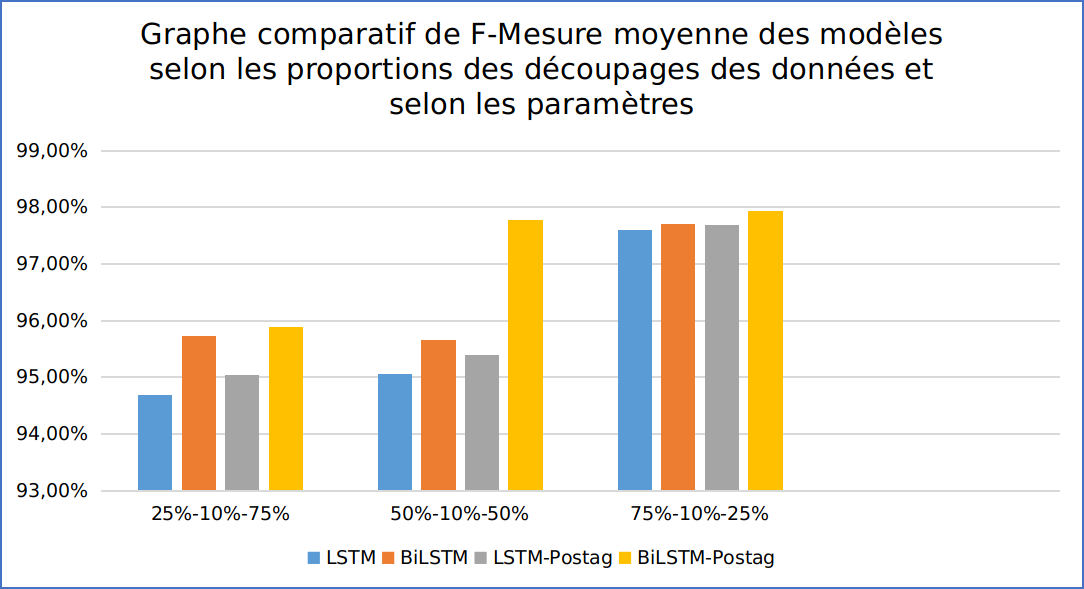
\includegraphics[width=.9\linewidth]{images/implementation/graphs.png} 
		\caption{Graphe comparatif selon les proportions des découpages des données et selon les paramètres.}
		\label{compare}
	\end{figure}
	\paragraph{}
	Nous pouvons remarquer l'impact de trois facteurs :
	\begin{itemize}
		\item \textbf{La taille de l'ensemble d'apprentissage} : 
		Systématiquement, le score F-Mesure moyen augmente avec la croissance du volume de données d'apprentissage. Cela laisse présager qu'avec plus de données le modèle pourrait mieux généraliser, ce qui éviterait de biaiser le modèle vers un type de données en particulier.
		
		\item \textbf{L'utilisation du contexte (LSTM contre BiLSTM)} : Le modèle BiLSTM donne de meilleur résultat lorsque l'information du contexte lui est accessible, ce qui confirme notre intuition. 
		
		\item \textbf{L'utilisation de l'étiquetage morphosyntaxique} : L'ajout de l'information sur la syntaxe de la requête semble aider le modèle à construire une meilleure représentation interne de la requête. Il ne voit pas un mot seulement à un instant $t$, mais plutôt la paire (mot,rôle syntaxique du mot dans la phrase). Cet ajout est conforme à notre explication théorique dans la section \ref{encoding}
	\end{itemize}
\section{Ontologie et manipulation du graphe d'état}
\paragraph{}Les ontologies déjà présentées dans la section \ref{onto1} ont été créées en utilisant Protégé. Elles ont été ensuite exportées en format Turtle\footnote{Turtle est une syntaxe pour l'écriture des triplets d'un graphe de connaissance avec RDF} afin de les exploiter dans la suite de ce travail en utilisant la bibliothèque RDFLib de Python.\\[6pt]
Les n\oe{}uds et les relations du graphe ont des identifiants entiers pour faciliter leur utilisation avec les réseaux de neurones. Une phase de transformation des URIs\footnote{Les URIs identifient de manière unique les ressources dans le web sémantique et sont également utilisés pour identifier les concepts et les relations dans les ontologies} en identifiants entiers s'avère nécessaire. L'ontologie comprend 61 n\oe{}uds et 13 relations. Contrairement au nombre de relations, le nombre de concepts augmente au cours du dialogue; de nouveaux n\oe{}uds sont introduits après chaque échange. Ceci nécessite de garder un ensemble d'identifiants non utilisés pour les associer pendant le dialogue. Le tableau suivant résume l'association des identifiants aux n\oe{}uds et relations des graphes.
\begin{table}[H]
	\begin{center}
		
		\begin{tabular}{|l|c|}
			\hline
			\textbf{Ressource} & \textbf{Valeurs des identifiants}\\
			\hline
			N\oe{}uds de l'ontologie & [1-61]\\
			\hline
			Relations de l'ontologie & [1-13]\\
			\hline
			N\oe{}uds créés pendant un dialogue & [62-256]\\
			\hline
		\end{tabular}
		\caption{Tableau des identifiants}\label{table_ids}
	\end{center}
\end{table}
\section{L'agent de dialogue}\label{DMReal}
\paragraph{}Nous avons proposé dans la partie conception \ref{DQL} deux architectures pour entraîner l'agent de dialogue. La première se compose de deux parties, un module pour encoder le graphe d'état et un autre pour décider l'action à prendre. Chacun est entraîné séparément. Les deux modules étant des réseaux de neurones, nous avons pensé à une deuxième architecture en les connectant pendant la phase d'apprentissage. Cette connexion permet à l'encodeur de graphe de choisir les parties du dialogue, représentées par le graphe d'état, à mémoriser afin de mieux estimer la fonction de récompense.
\subsection{Encodeur de graphe}
\paragraph{}Dans la première méthode, l'entraînement de l'encodeur se fait avec une architecture encodeur-décodeur en passant les triplets du graphe comme entrées et sorties de cette architecture.
\subsubsection{Implémentation}
\par Le réseau de neurones a été implémenté en utilisant la bibliothèque Keras de Python. Nous avons utilisé des cellules GRUs (Gated Reccurent Units \citep{Cho2014}) comme unités récurrentes pour l'encodeur et le décodeur vu leur efficacité comparable aux LSTMs tout en utilisant un seul vecteur d'état, ce qui les rend moins exigeants en mémoire. Comme notre tâche consiste à encoder un graphe dans un vecteur, la taille de ce dernier est très importante. Intuitivement, plus cette taille est grande plus le nombre de triplets qu'on peut y encoder est grand. D'où l'intérêt des cellules GRUs qui permettent d'utiliser de plus grands vecteurs d'état en moins d'espace mémoire que les LSTMs.
\paragraph{}La génération aléatoire des graphes de taille $t$ triplets se fait en suivant les étapes suivantes:
\begin{itemize}
	\item choisir un nombre de n\oe{}uds $nn$ aléatoire entre $2$ et $t+1$.
	\item choisir un nombre d'arcs $na$ aléatoire entre $1$ et $nn-1$.
	\item choisir $nn$ identifiants de n\oe{}uds et $na$ identifiants d'arcs aléatoirement de l'ensemble des identifiants possibles.
	\item créer les triplets en choisissant pour chaque triplet deux n\oe{}uds et un arc aléatoirement des ensembles résultats de l'étape précédente. 
\end{itemize}
\par Pendant l'apprentissage, le générateur choisit une taille pour le graphe inférieure à une taille maximale et crée un graphe en suivant les étapes sus-citées. Ce dernier est passé à l'encodeur-décodeur comme entrée et sortie désirée.
\subsubsection{Résultats et discussion}
\paragraph{}Pour estimer la capacité de l'encodeur du graphe, nous avons varié la taille maximale du graphe ainsi que le vecteur d'état du GRU. Les résultats sont présentés dans le figure suivante.
\begin{figure}[H] 
	\centering
	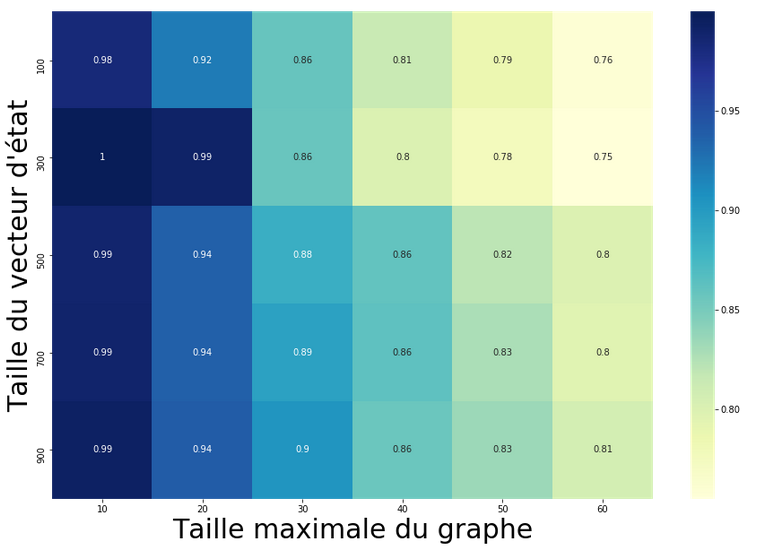
\includegraphics[width=0.95\linewidth]{images/Realisation/DM/heatmap.png}
	\caption{Variation de la précision en fonction de la taille maximale du graphe et la taille du vecteur d'état}\label{heatmap}
\end{figure}
\par Nous remarquons évidemment que la précision diminue avec l'augmentation de la taille maximale du graphe. Cependant, l'augmentation de la taille du vecteur encodant le graphe n'améliore pas beaucoup les résultats. Ceci peut être dû à la nature combinatoire du problème. En effet, la taille du graphe augmente exponentiellement en fonction du nombre de triplets. $nb$ et $t$ représentent respectivement le nombre de triplets possibles et la fonction correspondant à la taille du graphe le nombre de graphes possible. $t$ est définie par la fonction de récurrence suivante:
\[t(1) = nb\]
\[t(n+1) = t(n) \times nb\]
\par La première équation montre que le nombre de graphes possibles est égale au nombre de triplets possibles lorsque le graphe se compose d'un seul triplet. Tandis que la deuxième vient du fait que les graphes de taille $n+1$ peuvent être obtenus en combinant chaque graphe de taille $n$ avec tous les triplets possibles. Le résultat des deux équations est:
\[t(n) = nb^n\]
\par Pour pallier à ce problème, le graphe d'état peut être divisé en plusieurs sous-graphes, de façon à ce que chaque sous-graphe soit assez petit pour être encodé par l'un des encodeurs déjà entraînés. Ainsi, la concaténation de ces vecteurs peut être utilisée comme entrée pour le module suivant.
\subsection{Apprentissage par renforcement}
\paragraph{}Nous allons à présent présenter les deux méthodes citées dans la section \ref{DMReal}. La première consiste à utiliser le résultat de l'encodeur pour entraîner un réseau de neurones à estimer la récompense associée à chaque action possible. La deuxième, par contre, fait l'apprentissage des deux parties à la fois.
\par Nous utilisons un simulateur d'utilisateur pour communiquer avec l'agent de dialogue. Afin de simuler aussi les erreurs des modules précédents (reconnaissance automatique de la parole et compréhension du langage naturel), nous ajoutons un module qui insère du bruit dans les actions du simulateur. Sachant qu'une action utilisateur se compose de l'intention et des emplacements, ce dernier module prend donc deux valeurs de probabilités en paramètre; la probabilité de bruiter l'intention et celle de bruiter les emplacements. Dans la suite de ce travail, nous allons varier ces deux valeurs ainsi que la taille du vecteur d'état afin d'arriver à un compromis entre la robustesse face aux erreurs, la réussite des tâches utilisateur et l'utilisation de la mémoire.
\par Nous allons évaluer les différents résultats en comparant leur taux de succès qui est donné par le rapport entre le nombre de fois où l'agent arrive au but sur le nombre total d'essais. Un succès nécessite d'arriver au but dans un nombre d'échanges limite que nous avons estimé comme suit: 
\[limite = nb_{diff} \times 4 \times (1 + (pb_i + pb_e) \times 2) \]
\begin{itemize}
	\item limite: le nombre d'échanges maximal.
	\item $nb_{diff}$: le nombre de fichiers dans l'arborescence de départ en plus ou en moins par rapport à l'arborescence but.
	\item $pb_i$: la probabilité d'erreurs dans l'intention de l'utilisateur.
	\item $pb_e$: la probabilité d'erreurs dans les emplacements de l'action.
\end{itemize}
\par La première partie de l'équation, $nb_{diff} \times 4$, détermine une approximation du nombre d'actions nécessaire afin d'arriver au but; nous avons estimé qu'il faut un maximum de 4 échanges pour ajouter ou supprimer un fichier. La deuxième partie permet de prendre en compte les erreurs du simulateur. Sachant que le nombre moyen d'actions erronées en $n$ échanges est égal à $n \times (pb_i + pb_e)$, nous avons donc ajouté deux fois ce nombre. Ceci permet en premier lieu de ne pas compter les actions erronées dans la limite des échanges possibles, ainsi que d'ajouter des actions afin que l'agent puisse se retrouver dans la conversation après une erreur du simulateur.
\subsubsection{Apprentissage avec DQN déconnecté}
\paragraph{}Dans cette partie, nous utilisons un des encodeurs déjà entraînés dans la partie précédente. Nous avons donc choisi d'utiliser l'encodeur de taille 300 qui a été entraîné avec des graphes de taille maximale de 20. Nous avons varié le nombre de vecteurs utilisés ainsi que les probabilités d'erreurs du simulateur. Les résultats sont présentés dans le tableau \ref{table_results_dis}.
\definecolor{LightCyan}{rgb}{0.7,1,1}
\begin{table}[H]
	\begin{center}
		
		\begin{tabular}{|c|c|c|c|}
			\hline
			\textbf{Nombre de vecteurs} & \textbf{probabilité pb\textsubscript{i}} & \textbf{probabilité pb\textsubscript{e}} & \textbf{taux de réussite maximal}\\
			\hline
			4 & 0.25 & 0.3 & 0.25\\
			\hline
			4 & 0.05 & 0.2 & 0.59\\
			\hline
			\rowcolor{LightCyan}
			4 & 0.01 & 0.1 & 0.69\\
			\hline
			4 & 0 & 0 & 0.61\\
			\hline
			5 & 0.25 & 0.3 & 0.27\\
			\hline
			5 & 0.05 & 0.2 & 0.55\\
			\hline
			5 & 0.01 & 0.1 & 0.61\\
			\hline
			\textbf{5} & \textbf{0} & \textbf{0} & \textbf{0.72}\\
			\hline
			6 & 0.25 & 0.3 & 0.28\\
			\hline
			6 & 0.05 & 0.2 & 0.63\\
			\hline
			\rowcolor{LightCyan}
			6 & 0.01 & 0.1 & 0.69\\
			\hline
			6 & 0 & 0 & 0.7\\
			\hline
		\end{tabular}
		\caption{Taux de réussite en fonction des probabilités d'erreurs et du nombre de vecteurs d'état. Avec les probabilités pb\textsubscript{i} et pb\textsubscript{e}, les probabilités d'erreurs sur l'intention et les emplacements respectivement.}\label{table_results_dis}
	\end{center}
\end{table}
Le tableau \ref{table_results_dis} nous permet de conclure ce qui suit:
\begin{itemize}
	\item Évidemment, avec moins de probabilités d'erreurs, le réseau arrive à mieux reconnaître les motifs dans le vecteur d'état et leurs relations avec les récompenses du simulateur. Cependant, l'augmentation de la taille du vecteur n'améliore que légèrement les résultats; en calculant la moyenne des taux de réussite pour chaque nombre de vecteurs, les résultats sont comme suit: $53.5\%$ de taux de réussite pour quatre vecteurs, $53.75\%$ pour cinq vecteurs et $57.5\%$ pour six vecteurs.
	\item Le meilleur résultat a été obtenu en utilisant quatre vecteurs et sans erreurs avec un taux de réussite de $72\%$. En pratique, ce modèle ne s'adapte pas aux erreurs des modules précédents. Par conséquent, il se perd lorsqu'une erreur se produit et il n'arrive pas à se resituer dans la conversation.
	\item Avec des probabilités d'erreurs très élevées, le réseau n'arrive pas à apprendre et ne dépasse pas $28\%$ de taux de réussite.
	\item Les résultats les plus prometteurs, dans ce cas, sont ceux qui sont entraînés avec des probabilités d'erreurs proches de la réalité avec des taux de réussite acceptables. Dans ce cas, nous avons obtenu un taux de réussite de $69\%$ avec des probabilités d'erreurs de $1\%$ et $10\%$ sur les intentions et les emplacements respectivement.
\end{itemize}

\subsubsection{Apprentissage avec DQN connecté}
\paragraph{} Connecter le DQN avec l'encodeur devrait permettre de réduire la taille du vecteur d'état nécessaire. Comme pour la partie précédente, nous avons varié la taille du vecteur d'état ainsi que les probabilités des erreurs pour pouvoir par la suite comparer les deux approches proposées. 
\begin{table}[H]
	\begin{center}
		
		\begin{tabular}{|c|c|c|c|}
			\hline
			\textbf{Taille du vecteur d'état} & \textbf{probabilité pb\textsubscript{i}} & \textbf{probabilité pb\textsubscript{e}} & \textbf{taux de réussite maximal}\\
			\hline
			50 & 0.25 & 0.3 & 0.69\\
			\hline
			50 & 0.05 & 0.2 & 0.77\\
			\hline
			50 & 0.01 & 0.1 & 0.80\\
			\hline
			50 & 0 & 0 & 0.87\\
			\hline
			100 & 0.25 & 0.3 & 0.59\\
			\hline
			100 & 0.05 & 0.2 & 0.81\\
			\hline
			100 & 0.01 & 0.1 & 0.84\\
			\hline
			100 & 0 & 0 & 0.89\\
			\hline
			150 & 0.25 & 0.3 & 0.58\\
			\hline
			150 & 0.05 & 0.2 & 0.82\\
			\hline
			150 & 0.01 & 0.1 & 0.80\\
			\hline
			150 & \textbf{0} & \textbf{0} & \textbf{0.93}\\
			\hline
			200 & 0.25 & 0.3 & 0.59\\
			\hline
			200 & 0.05 & 0.2 & 0.82\\
			\hline
			\rowcolor{LightCyan}
			200 & 0.01 & 0.1 & 0.85\\
			\hline
			200 & 0 & 0 & 0.86\\
			\hline
		\end{tabular}
		\caption{Taux de réussite en fonction des probabilités d'erreurs et de la taille du vecteur d'état. Avec les probabilités pb\textsubscript{i} et pb\textsubscript{e}, les probabilités d'erreurs sur l'intention et les emplacements respectivement.}\label{table_results_con}
	\end{center}
\end{table}
\begin{itemize}
	\item Comme pour la méthode précédente, l'augmentation des probabilités d'erreurs diminue le taux de réussite en général.
	\item Le meilleur taux de réussite est toujours obtenu en faisant un apprentissage sans erreurs ce qui a donné $93\%$ de réussite.
	\item Pour des probabilités d'erreurs élevées, le taux de réussite diminue considérablement par rapport aux autres valeurs de probabilités.
	\item Le réseau arrive à reconnaître les motifs encodés aussi bien pour de petites tailles du vecteur d'état que pour de grandes tailles. Cette méthode permet effectivement de réduire la taille du vecteur encodant le graphe d'état par rapport à son prédécesseur.	
\end{itemize}

\subsubsection{Comparaison des approches et discussion}
\paragraph{}En comparant les deux méthodes, apprentissage avec DQN déconnecté et apprentissage avec DQN connecté, il est évident que la deuxième méthode est beaucoup plus efficace. Dans cette partie, nous allons donner de potentielles explications aux résultats trouvés en analysant les forces et faiblesses de chaque méthode. Nous allons analyser les méthodes par rapport à trois aspects: le taux de réussite, la vitesse d'apprentissage et la courbe d'apprentissage.
\subsubsection{Taux de réussite}\label{success_rate}
\paragraph{}Il est clair que connecter l'encodeur avec le réseau DQN a donné de meilleurs résultats. Ceci peut être dû aux facteurs suivants:
\begin{itemize}
	\item La difficulté de comprendre les motifs encodés séparément: En effet, la deuxième méthode permet au réseau de neurones d'apprendre à générer des motifs qui correspondent aux poids du réseau DQN.
	\item Deux états de dialogue lointains peuvent être encodés dans des vecteurs très proches en utilisant un encodeur séparé. Par exemple, il se peut que deux graphes soient similaires sauf pour un n\oe{}ud d'action qui est dans un graphe de type \textbf{Create\_node} et dans l'autre graphe \textbf{Delete\_node}. Dans ce cas, si l'encodeur les encode dans des vecteurs proches, le DQN aura des difficultés à distinguer les deux états. Par contre, en connectant l'encodeur avec le DQN, il peut observer les récompenses pour avoir l'information que certains n\oe{}uds sont plus importants que d'autres, les n\oe{}uds d'action par exemple, et qu'ils peuvent changer complètement l'état du vecteur.
	\item Les erreurs provenant de l'encodeur: Bien que la précision de l'encodeur obtenue était de $99\%$, en empilant 6 vecteurs encodés avec le même taux d'erreurs pour chacun et sachant que la probabilité d'erreur dans un vecteur est indépendante des autres, cette précision diminue à $96\%$.
\end{itemize}
\subsubsection{Vitesse d'apprentissage}
\paragraph{}Nous avons comparé les vitesses d'apprentissage des deux approches. En utilisant le réseau DQN séparé, ce dernier apprend avec une moyenne de \textbf{1013.15 instances/seconde}. De l'autre côté, le réseau connecté ne fait que \textbf{197.61 instances/seconde}. La raison derrière la lenteur de la deuxième approche revient à la nécéssité de refaire l'encodage de tout le graphe d'état de l'instance sauvegardée pendant les échanges avec le simulateur. Tandis que dans la deuxième approche, on ne sauvegarde que le vecteur déjà encodé.\\\\
Les temps des échanges avec le simulateur des deux approches sont proches puisqu'ils se comportent de la même manière dans ce cas. Les deux méthodes n'encodent que les nouveaux triplets arrivant dans le vecteur d'état précédent. 
\subsubsection{Courbe d'apprentissage}
\paragraph{}Enfin, nous comparons à présent les courbes d'apprentissage des deux méthodes. Celles-ci montrent le taux de réussite par rapport au nombre d'épisodes\footnote{Un épisode est un ensemble d'échanges agent-simulateur qui aboutit à un succès ou un échec}. La figure \ref{courbes} contient quatre courbes: deux courbes pour chaque méthode, avec et sans erreurs.
\begin{figure}[H] 
	\centering
	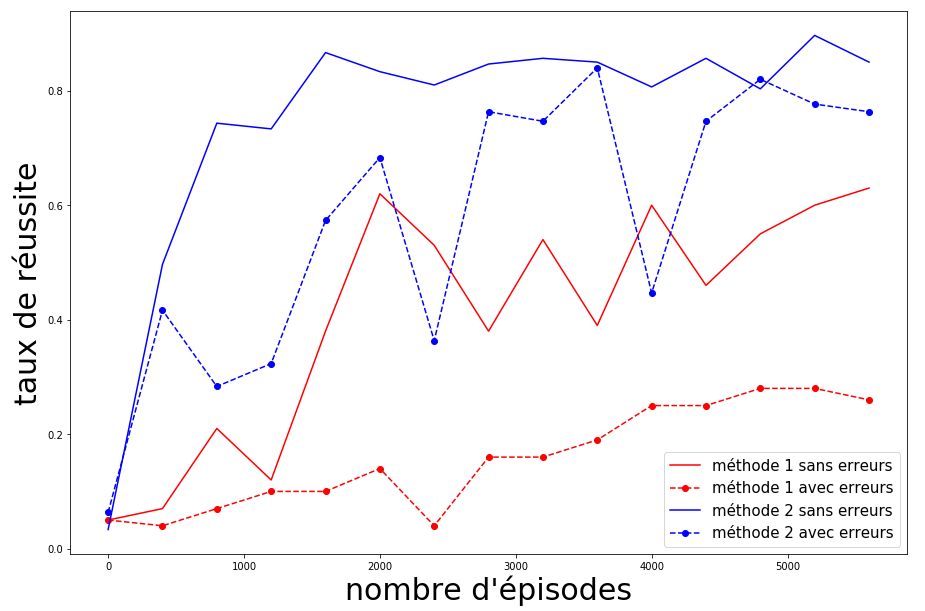
\includegraphics[width=0.95\linewidth]{images/Realisation/DM/courbes.png}
	\caption{Les courbes d'apprentissage des deux méthodes proposées avec et sans erreurs du simulateur d'utilisateur}\label{courbes}
\end{figure}
\paragraph{}Nous remarquons que la deuxième méthode arrive beaucoup plus rapidement à comprendre la fonction de récompense. Il s'avère donc que déconnecter le DQN de l'encodeur rend effectivement la tâche de trouver la relation entre les motifs des vecteurs d'états et les récompenses plus difficile.\\[6pt]
L'apprentissage peut être amélioré dans les deux cas, et surtout en ce qui concerne le premier, en utilisant un meilleur encodage des n\oe{}uds et des arcs du graphe. En effet, les n\oe{}uds sont actuellement encodés avec des identifiants entiers seulement, perdant ainsi les riches connaissances sémantiques qu'on peut extraire des relations du graphe. Un meilleur encodage serait d'utiliser des méthodes d'apprentissage semi-supervisé qui permettraient de donner aux n\oe{}uds proches un encodage similaire. Cette méthode permet d'éviter quelques problèmes que nous avons cités dans \ref{success_rate}, entre autres le problème d'encoder deux états lointains dans des vecteurs proches.

\section{Application Speech2Act}
\paragraph{}L'application Speech2Act relie les modules que nous avons implémentés dans un assistant qui aide à manipuler les fichiers de l'ordinateur avec la voix. Le schéma \ref{schema_app} montre les différentes parties que comporte l'application et les communications entre elles.
\begin{figure}[H] 
	\centering
	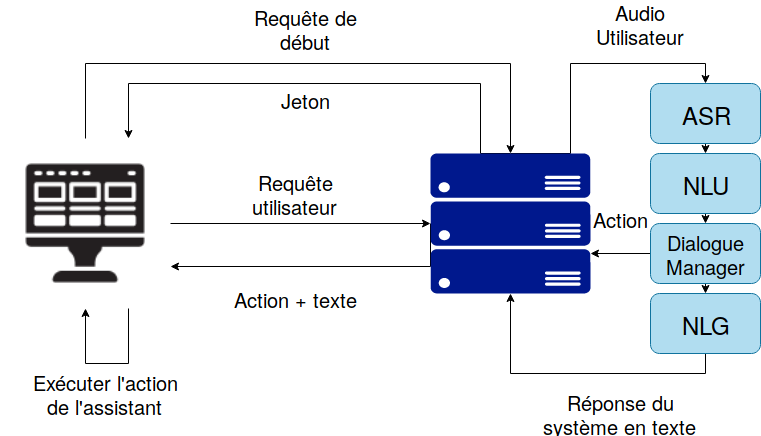
\includegraphics[width=0.95\linewidth]{images/Realisation/schema_app.png}
	\caption{Schéma général de l'application Speech2Act}\label{schema_app}
\end{figure}
\par L'application contient principalement deux parties: une partie frontend, avec laquelle l'utilisateur interagit, et une partie backend qui contient tous les modules que nous avons traités au cours de ce travail. Cette dernière partie se trouve dans un serveur qui répond aux requêtes de l'utilisateur. Les requêtes de l'utilisateur contiennent les données audio collectées par l'interface ainsi que les données du système sur lesquelles l'assistant peut agir. Quant-à la réponse du backend, elle est sous forme d'une action qui peut être exécutée par le côté client de l'application. Nous n'avons cependant pas encore traité les cas de permissions et les limites de ce que peut manipuler l'assistant. Néanmoins, nous avons limité l'espace des actions de l'assistant pour qu'il ne puisse agir que sur une arborescence de fichier test.
\subsection{Backend}
\paragraph{}Pour implémenter le backend, nous avons utilisé le micro-framework Flask qui permet d'écrire en Python le côté serveur d'une application. Les communications client-serveur de notre application se font comme suit:
\begin{itemize}
	\item Au lancement de l'application du côté client, celle-ci envoie une requête de début contenant l'état du système, dans notre cas une arborescence de fichiers. 
	\item Le backend lui répond avec un token (jeton) qui sera l'identifiant de cet utilisateur.
	\item Lorsque l'utilisateur parle à l'assistant, une requête est envoyée contenant son enregistrement audio. Alternativement, l'utilisateur peut introduire directement du texte qui sera envoyé dans la requête.
	\item Le backend reçoit le contenu de la requête. S'il s'agit d'un enregistrement audio, il le fait passer par le module de reconnaissance de la parole pour le convertir en texte.
	\item Le texte passe ensuite par le module de compréhension du langage qui est directement connecté avec le gestionnaire de dialogue. Ce dernier reçoit l'action résultat du module précédent et décide quelle action prendre selon l'état du système de l'utilisateur en question.
	\item L'action de l'assistant est transformée en langage naturel avant qu'elle ne soit envoyée à l'utilisateur.
	\item Le côté client de l'application reçoit le texte et l'action de l'assistant. Il exécute l'action et affiche le texte à l'utilisateur.
\end{itemize}

\subsection{Frontend}
\paragraph{}
Pour la réalisation de l'interface de l'application, nous avons opté pour une interface basée web (facilement exportable vers Desktop). Pour cela nous avons utilisé le framework VueJS augmenté par le plugin Vuetify. le résultat est une interface épurée et qui se veut simple et légère. L'utilisation d'un framework basé web permet de facilement créer des boucles d'éventements dont l'état interne est géré entièrement par le navigateur et le moteur VueJS. 

\begin{figure}[H]
	\centering
	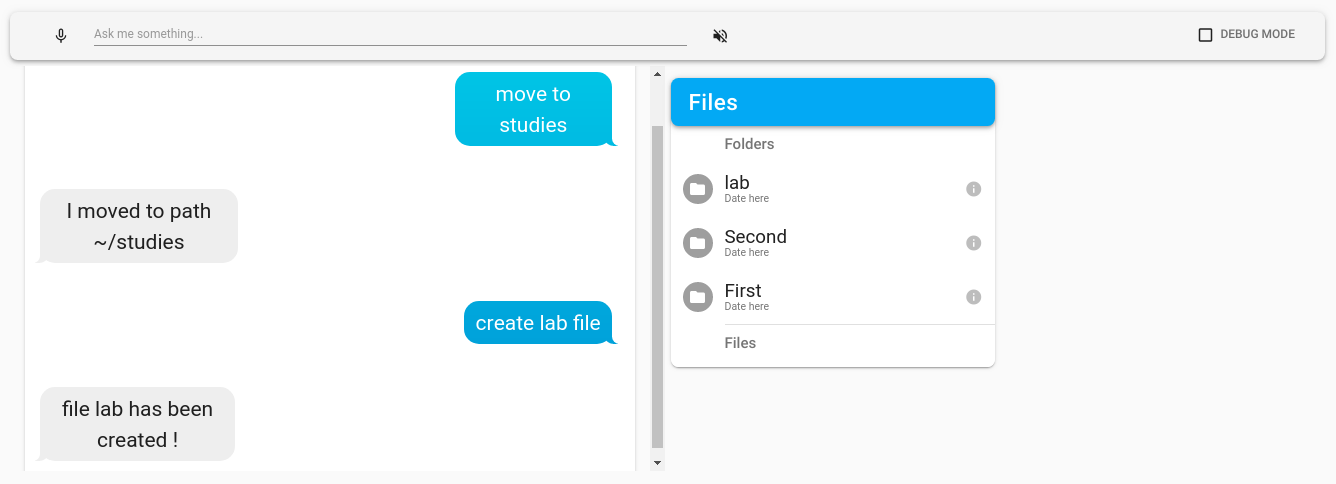
\includegraphics[width=\linewidth]{images/implementation/app_screens/main.png} 
	\caption{Interface principale de Speech2Act}
\end{figure} 

\par 
L'application se compose de quatre parties disposées sur une seule page web dynamiquement mise à jour au fur et à mesure du dialogue :

\begin{itemize}
	\item \textbf{Champ de saisie} : C'est une petite surface qui permet à l'utilisateur de communiquer avec le système. Il lui est possible bien entendu d'utiliser du texte ou bien de cliquer sur le bouton Microphone à gauche pour lancer des commandes vocales. Pour l'instant, c'est à l'utilisateur d'arrêter l'enregistrement de la commande ou bien d'attendre une période limite fixée à 7 secondes. Le bouton de volume permet d'activer ou non la réponse vocale du système (extensions de synthèse vocale). Le bouton tout à droite est réservé au mode Développeur pour analyser l'interaction entre le système et l'utilisateur.
	
	\item \textbf{Arborescence virtuelle} : C'est une petite fenêtre pour faciliter à l'utilisateur la mémorisation de l'environnement d'interaction. Cette fenêtre est dynamiquement mise à jour à travers le déroulement du dialogue et la manipulation des fichiers/répertoires.
	
	\begin{figure}[H]
		\centering
		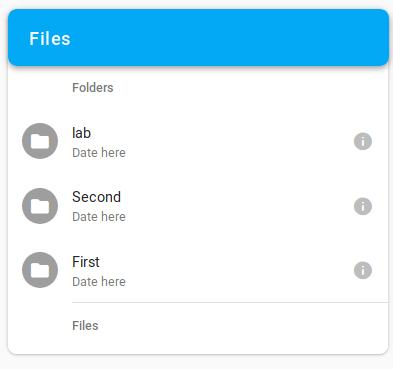
\includegraphics[width=.4\linewidth]{images/implementation/app_screens/tree.png}
		\caption{Fenêtre d'affichage de l'arborescence virtuelle}
	\end{figure} 
	
	\item \textbf{Champ de dialogue} : C'est là que vont résider toutes les informations sur le dialogue tout au long du cycle de vie de l'application. Il est mis à jour à chaque échange entre l'utilisateur et l'assistant Speech2Act. Il permet ainsi de garder trace de tous les échanges effectués et pouvoir à tout moment vérifier ou réutiliser des messages.
	\begin{figure}[H]
		\centering
		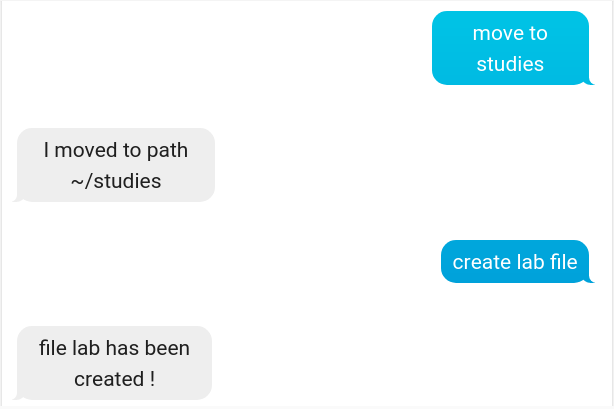
\includegraphics[width=.6\linewidth]{images/implementation/app_screens/dialog.png}
		\caption{Fenêtre de dialogue avec l'assistant}
	\end{figure} 
	
	\item \textbf{Fenêtre de Débogage} : C'est une option réservée aux développeurs pour faciliter les tests durant le développement. Toute réponse du serveur peut y être affichée pour peu qu'elle soit au format JSON sous la forme d'une réponse à une requête RESTFul. Pour le moment, il y est affiché l'intention de l'utilisateur avec son degré de confiance généré par Speech2Act, ainsi que les arguments de la requête (nom, type, positions ...).
	
	\begin{figure}[H]
		\centering
		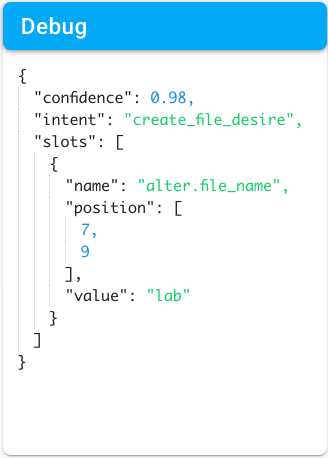
\includegraphics[width=.38\linewidth]{images/implementation/app_screens/debug.png}
		\caption{Fenêtre de Débogage}
	\end{figure} 

\end{itemize}
\section{Conclusion}
\paragraph{}
Au terme de ce chapitre, nous avons pu apprécier les fruits d'un long travail de conception. L'implémentation de certaines fonctionnalités a permis de mieux apprécier la complexité de la tâche qu'est le développement de Speech2Act. Chaque module a été soumis à une série de tests pour déterminer ses forces, faiblesses et limites. Une rapide analyse stipulant que pour un manque de données flagrant et un manque de ressources frustrant, Speech2Act a pu effectuer des petites tâches rudimentaires de manipulation du bureau sur un ordinateur et délivrer une mini-expérience de ce que peut être un véritable assistant virtuel intelligent.
